%!TEX TS-program = personallatex
%!TEX encoding = UTF-8 Unicode

% Le script utilisé pour compiler est :
%       xelatex --file-line-error --shell-escape --synctex=1

\documentclass[9pt, a4paper, obeyspaces]{extarticle}
% L'option 'openany' permet de démarrer un chapitre sur une page paire

% L'option 'obeyspaces' indique au paquetage hyperref de respecter les espaces dans les chemins \path ou \url.
% Par exemple : \path{ab cd} est écrit ab cd
% Sans cette option, \path{ab cd} est écrit abcd
% Voir : http://compgroups.net/comp.text.tex/space-in-path-hyperref-package


\usepackage{verbatim}

%-----------------------------------------------------------------------------------------------------------------------*
%                                                                                                                       *
%   E N C O D A G E    D E S    S O U R C E S     :     U T F 8                                                         *
%                                                                                                                       *
%-----------------------------------------------------------------------------------------------------------------------*

%--------------------------- Pour compilation XeLaTex
% http://www.tuteurs.ens.fr/logiciels/latex/xetex.html
\RequirePackage{etex}
\usepackage{fontspec}
\setmainfont{Verdana}[Ligatures=TeX]
\setmonofont{Courier}[Ligatures=NoCommon, Scale=0.95]
\setsansfont{Courier}[Ligatures=NoCommon, Scale=0.95]

%-----------------------------------------------------------------------------------------------------------------------*
%                                                                                                                       *
%   M I S E    E N    P A G E                                                                                           *
%                                                                                                                       *
%-----------------------------------------------------------------------------------------------------------------------*

%--- Latex demande ce paquetage pour mieux afficher le caractère "°" et \textquotesingle "'"
\usepackage{textcomp}

%--- Contrôle de l'indentation et de la séparation des paragraphes
\setlength{\parindent}{0pt} 
\setlength{\parskip}{1.1ex} % Reporté avant les chapitres

%--- Ajouter une séparation à la fin des itemize
%\let\EndItemize\enditemize
%\def\enditemize{\EndItemize\vspace{1.2ex}}

\usepackage[dvipsnames]{xcolor}

%--- Interligne 1,5 ligne
\usepackage{setspace}
\onehalfspacing
%\doublespacing

% Voir "Une courte introduction à Latex2e", § 6.4

%--- Marge gauche : 2,54 cm ; le paramètre \hoffset contient cette valeur, moins 1 pouce
%    \hoffset = 2,54 cm - 2,54 cm = 0 cm
\setlength{\hoffset}{0.cm}

%--- Marges supplémentaires, différenciées pour les pages gauches et droites ; ici, aucune.
\setlength{\oddsidemargin }{0 cm}
\setlength{\evensidemargin}{0 cm}

%--- Largeur du texte
%    \textwidth = 210 mm - 25.4 mm - 25.4 mm = 15,4 cm
\setlength{\textwidth}{15.92 cm}

%--- Marge haute : 2,54 cm ; le paramètre \voffset contient cette valeur, moins 1 pouce
%    \voffset = 2,54 cm - 2,54 cm = 0 cm
\setlength{\voffset}{0 cm}

%--- Distance entre la marge haute et l'en-tête : 0 cm
\setlength{\topmargin}{0 cm}

%--- Hauteur de l'en-tête de chaque page : 1 cm
\setlength{\headheight}{1 cm}

%--- Distance entre l'en-tête de chaque page et le corps : 0,5 cm
\setlength{\headsep}{0.5 cm}

%--- Hauteur du corps
%    \textheight = 29,7 cm - 2,54 cm - 2,8 cm - 1,5 cm = 22,6 cm
\setlength{\textheight}{22.86 cm}

%-----------------------------------------------------------------------------------------------------------------------*
%                                                                                                                       *
%   E X T E N S I O N S    P O U R    L ' É C R I T U R E    D E S     F O R M U L E S    M A T H É M A T I Q U E S     *
%                                                                                                                       *
%-----------------------------------------------------------------------------------------------------------------------*

%--- Extensions pour l'écriture des formules mathématiques
\usepackage{amsmath}
\usepackage{amssymb}
\usepackage{amsfonts}

%--- Paquetage "IEEEtrantools"
% Pour créer des tableaux d'équations, bien alignées
% Voir courte-intro-latex.pdf, page §3.5.2 page 83
\usepackage[retainorgcmds]{IEEEtrantools}

%-----------------------------------------------------------------------------------------------------------------------*

\usepackage{mdframed}

%-----------------------------------------------------------------------------------------------------------------------*
%                                                                                                                       *
%   P A Q U E T A G E    « L I S T I N G S »                                                                            *
%                                                                                                                       *
%-----------------------------------------------------------------------------------------------------------------------*

\usepackage{listings}

\lstset{
  basicstyle=\ttfamily\small,
  keywordstyle=\color{blue},
  commentstyle=\color{red},
  stringstyle=\color{orange},
  frame=l,
  backgroundcolor=\color{green!10},
  numberstyle=\ttfamily\small,
  xleftmargin=20pt
}

%-----------------------------------------------------------------------------------------------------------------------*
%                                                                                                                       *
%   H Y P E R R E F                                                                                                     *
%                                                                                                                       *
%-----------------------------------------------------------------------------------------------------------------------*

%--- Pour les hyperliens, et le contrôle de la génération PDF 
\usepackage[pagebackref]{hyperref}

\hypersetup{pdftitle      = {Python makefile}}
\hypersetup{pdfauthor     = {Pierre Molinaro}}

\hypersetup{colorlinks    = true}
\hypersetup{anchorcolor   = black}
\hypersetup{filecolor     = black}
\hypersetup{menucolor     = black}
\hypersetup{plainpages    = false}
\hypersetup{pdfstartview  = FitH}
\hypersetup{pdfpagelayout = OneColumn}
\hypersetup{linkcolor  = blue}
\hypersetup{urlcolor   = blue}
\hypersetup{citecolor  = blue}

%-----------------------------------------------------------------------------------------------------------------------*
%                                                                                                                       *
%   T I K Z    -    P G F                                                                                               *
%                                                                                                                       *
%-----------------------------------------------------------------------------------------------------------------------*

\usepackage{tikz}
\usetikzlibrary{calc}
\usepackage{pgfplots}
\usetikzlibrary{arrows}
\usetikzlibrary{decorations}
\usetikzlibrary{decorations.pathmorphing}
\usetikzlibrary{decorations.shapes}
\usetikzlibrary{shapes.callouts}
\usetikzlibrary{shapes.misc}
\usetikzlibrary{automata}
\usetikzlibrary{positioning}
\usepgflibrary{shapes.geometric}
\usepgfmodule{plot}

%-----------------------------------------------------------------------------------------------------------------------*
%                                                                                                                       *
%   Chiffres entourés (\ding{172} à \ding{211})                                                                         *
%                                                                                                                       *
%-----------------------------------------------------------------------------------------------------------------------*

\usepackage{pifont}

%-----------------------------------------------------------------------------------------------------------------------*
%                                                                                                                       *
%   E N - T Ê T E S    E T    P I E D S    D E    P A G E S                                                             *
%                                                                                                                       *
%-----------------------------------------------------------------------------------------------------------------------*

\usepackage{fancyhdr}
\pagestyle{fancy}

\usepackage{xcolor}

%------------------------------------------------------------------------------------------ RÉFÉRENCES À UNE SECTION
% Au lieu d'écrire \section{titre-section}, on écrit \sectionLabel{titre-section}{label-section}
\newcommand \sectionLabel[2]{\section{#1}\label{sec:#2}}


% \refSectionPage{label-section} ---> "section x.y page n"   où x.y est le n° de la section
\newcommand\refSectionPage[1]{\hyperref[sec:#1]{section \ref*{sec:#1} page \pageref{sec:#1}}}

%------------------------------------------------------------------------------------------ RÉFÉRENCES À UNE SUB-SECTION
% Au lieu d'écrire \subsection{titre-section}, on écrit \subsectionLabel{titre-section}{label-section}
\newcommand \subsectionLabel[2]{\subsection{#1}\label{subsec:#2}}


% \refSubsectionPage{label-section} ---> "section x.y page n"   où x.y est le n° de la sub-section
\newcommand\refSubsectionPage[1]{\hyperref[subsec:#1]{section \ref*{subsec:#1} page \pageref{subsec:#1}}}

%------------------------------------------------------------------------------------------ RÉFÉRENCES À UNE SUB-SUB-SECTION
% Au lieu d'écrire \subsubsection{titre-section}, on écrit \subsubsectionLabel{titre-section}{label-section}
\newcommand \subsubsectionLabel[2]{\subsubsection{#1}\label{subsubsec:#2}}


% \refSubsubsectionPage{label-section} ---> "section x.y page n"   où x.y est le n° de la sub-sub-section
\newcommand\refSubsubsectionPage[1]{\hyperref[subsubsec:#1]{section \ref*{subsubsec:#1} page \pageref{subsubsec:#1}}}

%-----------------------------------------------------------------------------------------------------------------------*
%                                                                                                                       *
%   R É F É R E N C E S   À   U N   T A B L E A U                                                                       *
%                                                                                                                       *
%-----------------------------------------------------------------------------------------------------------------------*

\usepackage{caption}

% Requires le "caption" package: \usepackage{caption}
\captionsetup[table]{labelfont=bf, labelsep=endash, name=Table}

% La référence au tableau "nom-du-tableau" est définie par \labelTableau{nom-du-tableau}
\newcommand\labelTableau[1]{\label{tab:#1}}
% Latex autorise deux types d'appel à une référence \ref{tab:nom-du-tableau} et \pageref{tab:nom-du-tableau}

% \refTableau{}{nom-du-tableau} ---> "tableau x.y"   où x.y est le n° du tableau
\newcommand\refTableau[1]{\hyperref[tab:#1]{table \ref*{tab:#1}}}

% \refTableauSansPrefixe{}{nom-du-tableau} ---> "x.y"   où x.y est le n° du tableau
\newcommand\refTableauSansPrefixe[1]{\hyperref[tab:#1]{\ref*{tab:#1}}}

% \refTableauPage{}{nom-du-tableau} ---> "tableau x.y page n"   où x.y est le n° du tableau
\newcommand\refTableauPage[1]{\hyperref[tab:#1]{table \ref*{tab:#1} page \pageref{tab:#1}}}

% \refTableauPageSansPrefixe{}{nom-du-tableau} ---> "x.y page n"   où x.y est le n° du tableau
\newcommand\refTableauPageSansPrefixe[1]{\hyperref[tab:#1]{\ref*{tab:#1} page \pageref{tab:#1}}}

%-----------------------------------------------------------------------------------------------------------------------*
%                                                                                                                       *
%   R É F É R E N C E S   À   U N E   F I G U R E                                                                       *
%                                                                                                                       *
%-----------------------------------------------------------------------------------------------------------------------*

\usepackage{ifthen}

% Requires le "caption" package: \usepackage{caption}
\captionsetup[figure]{labelfont=bf, labelsep=endash}

% La référence au tableau "nom-de-la-figure" est définie par \labelFigure{nom-de-la-figure}
\newcommand\labelFigure[1]{\label{fig:#1}}
% Latex autorise deux types d'appel à une référence \ref{fig:nom-de-la-figure} et \pageref{fig:nom-de-la-figure}

% \refFigure{}{nom-de-la-figure}   ---> "figure x.y"   où x.y est le n° de la figure
% \refFigure{z}{nom-de-la-figure}  ---> "figure x.y.z" où x.y est le n° de la figure
\newcommand\refFigure[2]{\hyperref[fig:#2]{figure \ref*{fig:#2}{\ifthenelse{\equal{#1}{}}{}{.#1}}}}

% \refFigureSansPrefixe{}{nom-de-la-figure}   ---> "x.y"   où x.y est le n° de la figure
% \refFigureSansPrefixe{z}{nom-de-la-figure}  ---> "x.y.z" où x.y est le n° de la figure
\newcommand\refFigureSansPrefixe[2]{\hyperref[fig:#2]{\ref*{fig:#2}{\ifthenelse{\equal{#1}{}}{}{.#1}}}}

% \refFigurePage{}{nom-de-la-figure}   ---> "figure x.y page n"   où x.y est le n° de la figure
% \refFigurePage{z}{nom-de-la-figure}  ---> "figure x.y.z page n" où x.y est le n° de la figure
\newcommand\refFigurePage[2]{\hyperref[fig:#2]{figure \ref*{fig:#2}{\ifthenelse{\equal{#1}{}}{}{.#1}} page \pageref{fig:#2}}}

% \refFigurePageSansPrefixe{}{nom-de-la-figure}   ---> "x.y page n"   où x.y est le n° de la figure
% \refFigurePageSansPrefixe{z}{nom-de-la-figure}  ---> "x.y.z page n" où x.y est le n° de la figure
\newcommand\refFigurePageSansPrefixe[2]{\hyperref[fig:#2]{\ref*{fig:#2}{\ifthenelse{\equal{#1}{}}{}{.#1}} page \pageref{fig:#2}}}

%-----------------------------------------------------------------------------------------------------------------------*
%                                                                                                                       *
%   C O N T R Ô L E    D E   L A   T A B L E   D E S   M A T I È R E S                                                  *
%                                                                                                                       *
%-----------------------------------------------------------------------------------------------------------------------*

% http://tex.stackexchange.com/questions/50471/question-about-indent-lengths-in-toc
\usepackage{tocloft}

%--- Gérer de l'indentation dans la table des matières
\cftsetindents{section}{0em}{2em}
\cftsetindents{subsection}{2em}{3em}
\cftsetindents{subsubsection}{4em}{5em}
%\cftsetindents{table}{0.0em}{3.0em}
%\cftsetindents{figure}{0.0em}{3.0em}

%--- Profondeur de la table des matières jusqu'au niveau 3 (subsubsection)
%\setcounter{tocdepth}{3}

%--- Numéroter les entrées jusqu'au niveau 3 (subsubsection)
%\setcounter{secnumdepth}{3}

%-----------------------------------------------------------------------------------------------------------------------*
%                                                                                                                       *
%   P A Q U E T A G E    « S U B F I G »                                                                                *
%                                                                                                                       *
%-----------------------------------------------------------------------------------------------------------------------*

% Grâce à ce paquetage, il est possible de placer plusieurs figures, tables, côte à côte.
% Voir http://en.wikibooks.org/wiki/LaTeX/Floats,_Figures_and_Captions
\usepackage{subfig} % Pour subfloat

%-----------------------------------------------------------------------------------------------------------------------*
%                                                                                                                       *
%   D É B U T    D U    D O C U M E N T                                                                                 *
%                                                                                                                       *
%-----------------------------------------------------------------------------------------------------------------------*

\begin{document} 

%-----------------------------------------------------------------------------------------------------------------------*
%                                                                                                                       *
%   T I T R E                                                                                                           *
%                                                                                                                       *
%-----------------------------------------------------------------------------------------------------------------------*

\title{\bf \Huge{ACAN2515 library for Arduino\\Version 2.0.4}}
\author{Pierre Molinaro}
\date {\today}

\maketitle

%-----------------------------------------------------------------------------------------------------------------------*
%                                                                                                                       *
%   T A B L E    D E S    M A T I È R E S                                                                               *
%                                                                                                                       *
%-----------------------------------------------------------------------------------------------------------------------*

\tableofcontents

%-----------------------------------------------------------------------------------------------------------------------*
%                                                                                                                       *
%   L E S    C H A P I T R E S                                                                                          *
%                                                                                                                       *
%-----------------------------------------------------------------------------------------------------------------------*

\newpage
\section{Versions}

\begin{center}
  \small
  \begin{tabular}{llp{11cm}}
    \textbf{Version} & \textbf{Date} & \textbf{Comment}\\
    2.0.4 & April 27, 2020 & Added \texttt{dataFloat} to \texttt{CANMessage} (thanks to \texttt{koryphon})\\
          &                & Added several forgotten \texttt{volatile}\\
    2.0.3 & January 9, 2020 & Interrupt pin is attached by \texttt{ACAN2515::beginWithoutFilterCheck} method only when there is configuration error (thanks to \texttt{mvSarma} for reporting this error). \\
    2.0.2 & June 15, 2019 & Added forgotten \texttt{ACAN2515::receiveBufferCount} and \texttt{ACAN2515::receiveBufferSize} methods (thanks to \texttt{Ede2016} for reporting this error). \\
          &               & ESP32: using \texttt{xSemaphoreGiveFromISR} instead of \texttt{xSemaphoreGive} in interrupt service routine. \\
    2.0.1 & April 19, 2019 & Fixed incorrect \texttt{SJW} setting. \\
    2.0.0 & February 19, 2019 & Added \texttt{SleepMode} mode (see \refSubsubsectionPage{mRequestedMode}). \\
          &                   & Added \texttt{ACAN2515::changeModeOnTheFly} function (\refSectionPage{changeModeOnTheFlyFunction}). \\
          &                   & Added \texttt{ACAN2515::setFiltersOnTheFly} functions (\refSectionPage{setFiltersOnTheFlyFunction}). \\
          &                   & Added \texttt{ACAN2515::end} function (\refSectionPage{endFunction}). \\
    1.1.3 & February 4, 2019 & Removed useless instructions in ESP32 sample codes. \\
    1.1.2 & February 3, 2019 & New option: no interrupt pin (\refSubsectionPage{noInterruptPin}). \\
          &                  & First release running on ESP32 (\refSubsectionPage{connectionESP32}). \\
    1.1.1 & January 20, 2019 & Updated documentation (\refSubsectionPage{defautFilterBehaviour}), as \texttt{mRolloverEnable} is \texttt{true} by default (thanks to \texttt{PatrykSSS} for reporting this documentation error).\\
          &                   & Added \texttt{ACAN2515::receiveBufferPeakCount} method, forgotten in previous releases (thanks to \texttt{qwec01} for reporting this bug).\\
          &                   & New error flag: \texttt{kCannotAllocateReceiveBuffer}, \refSubsubsectionPage{kCannotAllocateReceiveBuffer}.\\
          &                   & New error flag: \texttt{kCannotAllocateTransmitBuffer0}, \refSubsubsectionPage{kCannotAllocateTransmitBuffer0}.\\
          &                   & New error flag: \texttt{kCannotAllocateTransmitBuffer1}, \refSubsubsectionPage{kCannotAllocateTransmitBuffer1}.\\
          &                   & New error flag: \texttt{kCannotAllocateTransmitBuffer2}, \refSubsubsectionPage{kCannotAllocateTransmitBuffer2}.\\
    1.1.0 & November 24, 2018 & \texttt{ACAN2515Settings::CANBitSettingConsistency} now returns an \texttt{uint16\_t}. \\
          &                   & Compatibility with \texttt{ACAN2515Tiny} library.\\
    1.0.4 & November 23, 2018 & BugFix: transmit buffer \#2 size setting. \\
          &                   & Transmit and send buffers properties are now \texttt{uint16\_t} (instead of \texttt{uint32\_t}), for saving memory. \\
          &                   & \texttt{ACAN2515::begin} now returns an \texttt{uint16\_t} (instead of \texttt{uint32\_t}).\\
          &                   & New \texttt{ACAN2515Settings} constructor with explicit bit rate settings (see \refSubsectionPage{explicitCANbitSettings} and \texttt{LoopBackDemoBitRateSettings} demo sketch).\\
    1.0.3 & November 3, 2018 & Correct setting of \texttt{rtr} and \texttt{ext} properties on message receive (thanks to Arjan-Woltjer for having fixed this bug, \url{https://github.com/pierremolinaro/acan2515/pull/1}). \\
    1.0.1 & October 23, 2018 & Workaround external interrupt masking for Teensy 3.5 / 3.6.\\
          &                  & Use of a lambda function for interrupt service routine. \\
    1.0.0 & October 12, 2018 & Initial release. \\
  \end{tabular}
\end{center}

{\bf Note from updating from 1.0.x.}

In 1.0.x, the \texttt{ACAN2515RequestedMode} and \texttt{ACAN2515CLKOUT\_SOF} were autonomous enumeration classes. From 1.1.x, they are embedded in the \texttt{ACAN2515Settings} class. Consequently, the correspondant \texttt{ACAN2515Settings} property settings should be modified accordingly; for example:

{ \small\begin{lstlisting}[language=c++]
  settings.mRequestedMode = ACAN2515RequestedMode::LoopBackMode ; // In 1.0.x
\end{lstlisting}}

should be rewritten as:
{ \small\begin{lstlisting}[language=c++]
  settings.mRequestedMode = ACAN2515Settings::LoopBackMode ; // In 1.1.x
\end{lstlisting}}



\section{Features}

The \texttt{ACAN2515} library is a MCP2515 CAN ("Controller Area Network") Controller driver for any board running Arduino. It has been designed to make it easy to start and to be easily configurable:
\begin{itemize}
  \item default configuration sends and receives any frame -- no default filter to provide;
  \item efficient built-in CAN bit settings computation from user bit rate;
  \item user can fully define its own CAN bit setting values;
  \item all reception filter registers are easily defined (2 mask registers, 6 acceptance registers);
  \item reception filters accept call back functions;
  \item driver transmit buffer sizes are customisable;
  \item driver receive buffer size is customisable;
  \item overflow of the driver receive buffer is detectable;
  \item \emph{loop back}, \emph{self reception}, \emph{listing only} MCP2515 controller modes are selectable.
\end{itemize}



\section{Data flow}

The \refFigure{}{figureStructureStationCAN} illustrates message flow for sending and receiving CAN messages.

\begin{figure}[!ht]
  \small
  \centering
  \begin{tikzpicture}[line cap=round, line join=round, >=stealth]
  %--- User code
    \draw[very thick, fill=lightgray!25] (0.5, 12) -- ++(0, -1.5) -- ++ (14.5, 0) -- ++ (0, 1.5) ;
    \draw (7.5, 11.25) node {\bf\emph{User code}};
  %--- ACAN2515 driver
    \draw[very thick, fill=lightgray!25] (0.5, 7) rectangle ++ (14.5, 3);
    \draw (7.5, 10) node[below] {\bf\emph{ACAN2515 driver}};
    \draw (12.75, 10.5) node[above] {\begin{tabular}{c}\texttt{available}\\ \texttt{receive}\\ \texttt{dispatchReceivedMessage}\end{tabular}};
    \draw (2.5, 10.5) node[above] {\texttt{tryToSend}};
  %--- MCP2515 controller
    \draw[very thick, fill=lightgray!25] (0.5, 0.5) rectangle ++ (14.5, 6);
    \draw (7.5, 3.5) node {\bf\emph{MCP2515}};
  % Flèches
    \draw[<-, very thick] (2.5, 6) -- ++ (0, 1.5) ;
    \draw[<-, very thick] (6.0, 6) -- ++ (0, 1.5) ;
    \draw[<-, very thick] (9.5, 6) -- ++ (0, 1.5) ;
    \draw[->, very thick] (2.5, 4.5) -- ++ (0, -2.5) ;
    \draw[->, very thick] (6, 4.5) -- ++ (0, -2.5) ;
    \draw[->, very thick] (9.5, 4.5) -- ++ (0, -2.5) ;
    \draw[<-, very thick] (13, 2.5) -- ++ (0, -.5) ;
    \draw[<-, very thick] (13, 4.5) -- ++ (0, -.5) ;
    \draw[->, very thick] (13, 6) -- ++ (0, 1.5) ;
    \draw[->, very thick] (13, 9) -- ++ (0, 1.5) ;
    \draw[<-, very thick] (2.5, 9) -- ++ (0, 1.5) ;
    \draw[->, very thick] (2.5, 9.5) -- ++ (3.5, 0) -- ++ (0, -.5) ;
    \draw[->, very thick] (6, 9.5) -- ++ (3.5, 0) -- ++ (0, -.5) ;
%    \draw (5.25, 9.5) node[above]{\footnotesize\emph{remote frame}} ;
%    \draw (3, 9.25) node[left]{\footnotesize\emph{idx == 0}} ;
  %  Driver transmit FIFO 0
    \draw[fill=white] (1, 7.5) rectangle ++ (3, 1.5);
    \draw (2.5, 8.25) node {\begin{tabular}{c}\emph{Driver}\\ \emph{Transmit Buffer 0}\\ \emph{(FIFO)}\end{tabular}};
  %  Driver transmit FIFO 1
    \draw[fill=white] (4.5, 7.5) rectangle ++ (3, 1.5);
    \draw (6, 8.25) node {\begin{tabular}{c}\emph{Driver}\\ \emph{Transmit Buffer 1}\\ \emph{(FIFO)}\end{tabular}};
  %  Driver transmit FIFO 2
    \draw[fill=white] (8, 7.5) rectangle ++ (3, 1.5);
    \draw (9.5, 8.25) node {\begin{tabular}{c}\emph{Driver}\\ \emph{Transmit Buffer 2}\\ \emph{(FIFO)}\end{tabular}};
  %  Driver receive FIFO
    \draw[fill=white] (11.5, 7.5) rectangle ++ (3, 1.5);
    \draw (13, 8.25) node {\begin{tabular}{c}\emph{Driver}\\ \emph{Reception Buffer}\\ \emph{(FIFO)}\end{tabular}};
  % Protocol engine
    \draw[fill=white] (1, 1) rectangle ++ (13.5, 1);
    \draw (7.75, 1.5) node {\emph{CAN Protocol Engine}};
  % TxD
    %\draw (6.25, .5) node[above] {\texttt{CAN Tx}};
    \draw[->] (6.75, 1) -- ++ (0, -1) ;
    \draw (6.75, 0.5) node[fill=white, draw] {\texttt{TXCAN}};
  % RxD
    \draw[<-] (8.75, 1) -- ++ (0, -1) ;
    \draw (8.75, 0.5) node[fill=white, draw] {\texttt{RXCAN}};
  %  transmit data Buffer 0
    \draw[fill=white] (1, 4.5) rectangle ++ (3, 1.5);
    \draw (2.5, 5.25) node {\tt TXB0};
  %  transmit data Buffer 1
    \draw[fill=white] (4.5, 4.5) rectangle ++ (3, 1.5);
    \draw (6, 5.25) node {\tt TXB1};
  %  transmit data Buffer 2
    \draw[fill=white] (8, 4.5) rectangle ++ (3, 1.5);
    \draw (9.5, 5.25) node {\tt TXB2};
  %  Rx Filtres de réception
    \draw[fill=white] (11.5, 2.5) rectangle ++ (3, 1.5);
    \draw (13, 3.25) node {\emph{Reception filters}};
  %  Rx Buffers
    \draw[fill=white] (11.5, 4.5) rectangle ++ (3, 1.5);
    \draw (13, 5.25) node {\emph{Reception Registers}};
  \end{tikzpicture}
  \caption{Message flow in \texttt{ACAN2515} driver and \texttt{MCP2515} CAN Controller}
  \labelFigure{figureStructureStationCAN}
\end{figure}




{\bf Sending messages.} A message is defined by an instance of \texttt{CANMessage} class. For sending a message, user code calls the \texttt{tryToSend} method -- see \refSectionPage{sendingFrames}, and the \texttt{idx} property of the sent message specifies a transmit buffer. The ACAN2515 driver defines 3 transmit buffers, each of them corresponding to the one of the 3 \texttt{MCP2515} transmit buffers (\texttt{TXB0}, \texttt{TXB1}, \texttt{TXB2}). These buffers can contain at most one message. The message is  transfered in a driver transmit buffer before to be moved by the interrupt service routine into the corresponding MCP2515 transmit buffer. The size of the \emph{Driver Transmit Buffer 0} is 16 by default, the size of the \emph{Driver Transmit Buffer 1} and \emph{Driver Transmit Buffer 1} are zero by default  -- see \refSubsectionPage{driverTransmitBufferSize} for changing the default values.



{\bf Receiving messages.} The MCP2515 \emph{CAN Protocol Engine} transmits all correct frames to the \emph{reception filters}. By default, they are configured as pass-all, see \refSectionPage{acceptanceFilters} for configuring them. Messages that pass the filters are stored in the \emph{Reception Registers} (\texttt{RXB0} and \texttt{RXB1}). The interrupt service routine transfers the messages from these registers to the \emph{Driver Receive Buffer}. The size of the \emph{Driver Receive Buffer} is 32 by default -- see \refSubsectionPage{driverReceiveBufferSize} for changing the default value. Three user methods are available:
\begin{itemize}
  \item the \texttt{available} method returns \texttt{false} if the \emph{Driver Receive Buffer} is empty, and \texttt{true} otherwise;
  \item the \texttt{receive} method retrieves messages from the \emph{Driver Receive Buffer} -- see \refSectionPage{UsingReceiveMethod};
  \item the \texttt{dispatchReceivedMessage} method if you have defined the reception filters that name a call-back function -- see \refSectionPage{UsingDispatchMethod}.
\end{itemize}

{\bf Sequentiality.} The \texttt{ACAN2515} driver and the configuration of the \texttt{MCP2515} controller can ensure sequentiality of data messages\footnote{Sequentiality means that if an user program calls \texttt{tryToSend} first for a message $M_1$ and then for a message $M_2$, the message $M_1$ will be always retrieved by \texttt{receive} or \texttt{dispatchReceivedMessage} before the message $M_2$.}, under some conditions. The driver ensures the sequentiality of the emissions, provided that you use only one transmit buffer: if an user program calls \texttt{tryToSend} first for a message $M_1$ specifying the $B_i$ buffer and then for a message $M_2$ specifying the same buffer, the driver ensures that $M_1$ will be sent on the CAN bus before $M_2$. However, if $M_2$ specifies an other buffer, there is no guarantee that $M_1$ will appear on the bus before $M_2$. In reception, the driver ensures sequentiality based on the reception filters: if a received message $M_1$ passes a given filter, and then a received message $M_2$ passes the same filter, then the messages are retrieved in this order by the \texttt{receive} or the \texttt{dispatchReceivedMessage} methods.



\section{A simple example: \texttt{LoopBackDemo}}

The following code is a sample code for introducing the \texttt{ACAN2515} library, extracted from the \texttt{LoopBackDemo} sample code included in the library distribution. It runs natively on any Arduino compatible board, and is easily adaptable to any microcontroller supporting \texttt{SPI}. It demonstrates how to configure the driver, to send a CAN message, and to receive a CAN message.

Note: this code runs without any CAN transceiver (the \texttt{TXCAN} and \texttt{RXCAN} pins of the \texttt{MCP2515} are left open), the \texttt{MCP2515} is configured with the \emph{loop back} setting on.

{ \small\begin{lstlisting}[language=c++]
#include <ACAN2515.h>
\end{lstlisting}}

This line includes the \texttt{ACAN2515} library.

{ \small\begin{lstlisting}[language=c++]
static const byte MCP2515_SCK = 27 ; // SCK input of MCP2515 
static const byte MCP2515_SI  = 28 ; // SI input of MCP2515  
static const byte MCP2515_SO  = 39 ; // SO output of MCP2515 
\end{lstlisting}}
Define the \texttt{SPI} alternate pins. This is actually required if you uses \texttt{SPI} alternate pins.


{ \small\begin{lstlisting}[language=c++]
static const byte MCP2515_CS  = 20 ; // CS input of MCP2515 
static const byte MCP2515_INT = 37 ; // INT output of MCP2515
\end{lstlisting}}
Define the pins connected to $\overline{\texttt{CS}}$ and $\overline{\texttt{INT}}$ pins.




{ \small\begin{lstlisting}[language=c++]
ACAN2515 can (MCP2515_CS, SPI, MCP2515_INT) ;
\end{lstlisting}}
Instanciation of the \texttt{ACAN2515} library, declaration and initialization of the \texttt{can} object that implements the driver. The constructor names: the number of the pin connected to the $\overline{\texttt{CS}}$ pin, the \texttt{SPI} object (you can use \texttt{SPI1}, \texttt{SPI2}, …), the number of the pin connected to the $\overline{\texttt{INT}}$ pin.



{ \small\begin{lstlisting}[language=c++]
static const uint32_t QUARTZ_FREQUENCY = 16 * 1000 * 1000 ; // 16 MHz
\end{lstlisting}}

Specifies the frequency of the \texttt{MCP2515} quartz.








{ \small\begin{lstlisting}[language=c++]
void setup () {
//--- Switch on builtin led
  pinMode (LED_BUILTIN, OUTPUT) ;
  digitalWrite (LED_BUILTIN, HIGH) ;
//--- Start serial
  Serial.begin (38400) ;
//--- Wait for serial (blink led at 10 Hz during waiting)
  while (!Serial) {
    delay (50) ;
    digitalWrite (LED_BUILTIN, !digitalRead (LED_BUILTIN)) ;
  }
\end{lstlisting}}
Builtin led is used for signaling. It blinks led at 10 Hz during until serial monitor is ready.



{ \small\begin{lstlisting}[language=c++]
  SPI.begin () ;
\end{lstlisting}}
You should call \texttt{SPI.begin}. Many platforms define alternate pins for SPI. On Teensy 3.x (\refSubsectionPage{TeensyAlternatePins}), selecting alternate pins should be done before calling \texttt{SPI.begin}, on Adafruit Feather M0 (\refSubsectionPage{AdafruitFeatherM0AlternatePins}), this should be done after. Calling \texttt{SPI.begin} explicitly allows you to fully handle alternate pins.

{ \small\begin{lstlisting}[language=c++]
  ACAN2515Settings settings (QUARTZ_FREQUENCY, 125 * 1000) ;
\end{lstlisting}}

Configuration is a four-step operation. This line is the first step. It instanciates the \texttt{settings} object of the \texttt{ACAN2515Settings} class. The constructor has two parameters: the \texttt{MCP2515} quartz frequency, and the desired CAN bit rate (here, 125 kb/s). It returns a \texttt{settings} object fully initialized with CAN bit settings for the desired bit rate, and default values for other configuration properties.






{ \small\begin{lstlisting}[language=c++]
  settings.mRequestedMode = ACAN2515Settings::LoopBackMode ;
\end{lstlisting}}
This is the second step. You can override the values of the properties of \texttt{settings} object. Here, the \texttt{mRequestedMode} property is set to \texttt{LoopBackMode} -- its value is \texttt{NormalMode} by default. Setting this property enables \emph{loop back}, that is you can run this demo sketch even it you have no connection to a physical CAN network. The \refSubsectionPage{propertiesACAN2515Settings} lists all properties you can override.





{ \small\begin{lstlisting}[language=c++]
  const uint16_t errorCode = can.begin (settings, [] { can.isr () ; }) ;
\end{lstlisting}}
This is the third step, configuration of the \texttt{can} driver with \texttt{settings} values. The driver is configured for being able to send any (standard / extended, data / remote) frame, and to receive all (standard / extended, data / remote) frames. If you want to define reception filters, see \refSectionPage{acceptanceFilters}. The second argument is the \emph{interrupt service routine}, and is defined by a C++ lambda expression\footnote{\url{https://en.cppreference.com/w/cpp/language/lambda}}. See \refSubsectionPage{isrExplicit} for using a function instead.





{ \small\begin{lstlisting}[language=c++]
  if (errorCode != 0) {
    Serial.print ("Configuration error 0x") ;
    Serial.println (errorCode, HEX) ;
  }
}
\end{lstlisting}}
Last step: the configuration of the \texttt{can} driver returns an error code, stored in the \texttt{errorCode} constant. It has the value $0$ if all is ok -- see \refSubsectionPage{errorCodeMethodBegin}.








{ \small\begin{lstlisting}[language=c++]
static uint32_t gBlinkLedDate = 0 ;
static uint32_t gReceivedFrameCount = 0 ;
static uint32_t gSentFrameCount = 0 ;
\end{lstlisting}}
The \texttt{gSendDate} global variable is used for sending a CAN message every 2 s. The \texttt{gSentCount} global variable counts the number of sent messages. The \texttt{gReceivedCount} global variable counts the number of received messages.



{ \small\begin{lstlisting}[language=c++]
void loop() {
  CANMessage frame ;
\end{lstlisting}}
The \texttt{message} object is fully initialized by the default constructor, it represents a standard data frame, with an identifier equal to $0$, and without any data -- see \refSectionPage{CANMessageClass}. 







{ \small\begin{lstlisting}[language=c++]
  if (gBlinkLedDate < millis ()) {
    gBlinkLedDate += 2000 ;
    digitalWrite (LED_BUILTIN, !digitalRead (LED_BUILTIN)) ;
    const bool ok = can.tryToSend (frame) ;
    if (ok) {
      gSentFrameCount += 1 ;
      Serial.print ("Sent: ") ;
      Serial.println (gSentFrameCount) ;
    }else{
      Serial.println ("Send failure") ;
    }
  }
\end{lstlisting}}
We try to send the data message. Actually, we try to transfer it into the \emph{Driver transmit buffer}. The transfer succeeds if the buffer is not full. The \texttt{tryToSend} method returns \texttt{false} if the buffer is full, and \texttt{true} otherwise. Note the returned value only tells if the transfer into the \emph{Driver transmit buffer} is successful or not: we have no way to know if the frame is actually sent on the the CAN network. Then, we act the successfull transfer by setting \texttt{gSendDate} to the next send date and incrementing the \texttt{gSentCount} variable. Note if the transfer did fail, the send date is not changed, so the \texttt{tryToSend} method will be called on the execution of the \texttt{loop} function.


{ \small\begin{lstlisting}[language=c++]
  if (can.available ()) {
    can.receive (frame) ;
    gReceivedFrameCount ++ ;
    Serial.print ("Received: ") ;
    Serial.println (gReceivedFrameCount) ;
  }
}
\end{lstlisting}}
As the \texttt{MCP2515} controller is configured in \emph{loop back} mode, all sent messages are received. The \texttt{receive} method returns \texttt{false} if no message is available from the \emph{driver reception buffer}. It returns \texttt{true} if a message has been successfully removed from the \emph{driver reception buffer}. This message is assigned to the \texttt{message} object. If a message has been received, the \texttt{gReceivedCount} is incremented ans displayed.





\sectionLabel{The \texttt{CANMessage} class}{CANMessageClass}

{\bf Note. } The \texttt{CANMessage} class is declared in the \texttt{CANMessage.h} header file. The class declaration is protected by an include guard that causes the macro \texttt{GENERIC\_CAN\_MESSAGE\_DEFINED} to be defined. The ACAN\footnote{The ACAN driver is a CAN driver for FlexCAN modules integrated in the Teensy 3.x microcontrollers, \url{https://github.com/pierremolinaro/acan}.} (version 1.0.3 and above) driver, the ACAN2517\footnote{The ACAN2517 driver is a CAN driver for the \texttt{MCP2517} CAN controller, \url{https://github.com/pierremolinaro/acan2517}.} driver contain an identical \texttt{CANMessage.h} file header, enabling using ACAN driver, ACAN2515 driver and ACAN2517 driver in a same sketch.

A \emph{CAN message} is an object that contains all CAN frame user informations. All properties are initialized by default, and represent a standard data frame, with an identifier equal to $0$, and without any data.

{ \small\begin{lstlisting}[language=c++]
class CANMessage {
  public : uint32_t id = 0 ;  // Frame identifier
  public : bool ext = false ; // false -> standard frame, true -> extended frame
  public : bool rtr = false ; // false -> data frame, true -> remote frame
  public : uint8_t idx = 0 ;  // This field is used by the driver
  public : uint8_t len = 0 ;  // Length of data (0 ... 8)
  public : union {
    uint64_t data64        ; // Caution: subject to endianness
    uint32_t data32 [2]    ; // Caution: subject to endianness
    uint16_t data16 [4]    ; // Caution: subject to endianness
    float    dataFloat [2] ; // Caution: subject to endianness
    uint8_t  data   [8] = {0, 0, 0, 0, 0, 0, 0, 0} ;
  } ;
} ;
\end{lstlisting}}

Note the message datas are defined by an {\bf\texttt{union}}. So message datas can be seen as height bytes, four 16-bit unsigned integers, two 32-bit, one 64-bit or two 32-bit floats. Be aware that multi-byte integers and floats are subject to endianness (Cortex M7 processor of Teensy 4.x are little-endian).

The \texttt{idx} property is not used in CAN frames, but:
\begin{itemize}
  \item for a received message, it contains the acceptance filter index (see \refSectionPage{UsingDispatchMethod});
  \item on sending messages, it is used for selecting the transmit buffer (see \refSubsectionPage{tryToSendMethod}).
\end{itemize}









\section{Connecting a \texttt{MCP2515} to your microcontroller}


Connecting a \texttt{MCP2515} requires 5 pins (\refFigure{}{figureHardwareSPI}):
\begin{itemize}
  \item hardware SPI requires you use dedicaced pins of your microcontroller. You can use alternate pins (see below), and if your microcontroller supports several hardware SPIs, you can select any of them;
  \item connecting the $\overline{\tt CS}$ signal requires one digital pin, that the driver configures as an \texttt{OUTPUT} ;
  \item connecting the $\overline{\tt INT}$ signal requires one other digital pin, that the driver configures as an external interrupt input; so this pin should have interrupt capability (checked by the \texttt{begin} method of the driver object).
\end{itemize}

\begin{figure}[!ht]
  \small
  \centering
  \begin{tikzpicture}[line cap=round, line join=round, >=stealth]
  %--- Microcontroller
    \draw[very thick, fill=lightgray!25] (-1.5, 0) -- ++(5.5, 0)  -- ++(0, 3) -- ++ (-5.5, 0) ;
    \draw (0, 1.5) node {\bf\emph{Microcontroller}};
  %--- MCP2515
    \draw[very thick, fill=lightgray!25] (12, 0) -- ++(-4, 0)  -- ++(0, 3) -- ++ (4, 0) ;
    \draw (10.5, 1.5) node {\bf\emph{MCP2515}};
  %--- INT
    \draw[<-, thick] (4, 2.5) -- ++ (4, 0) ;
    \draw (8, 2.5) node[right] {$\overline{\tt INT}$};
    \draw (4, 2.5) node[left] {\tt MCP2515\_INT};
  %--- CS
    \draw[->, thick] (4, 2) -- ++ (4, 0) ;
    \draw (8, 2) node[right] {$\overline{\tt CS}$};
    \draw (4, 2) node[left] {\tt MCP2515\_CS};
  %--- SCK
    \draw[->, thick] (4, 1.5) -- ++ (4, 0) ;
    \draw (8, 1.5) node[right] {\tt SCK};
    \draw (4, 1.5) node[left] {\tt SCK};
  %--- SI
    \draw[->, thick] (4, 1) -- ++ (4, 0) ;
    \draw (8, 1) node[right] {\tt SI};
    \draw (4, 1) node[left] {\tt MOSI};
  %--- SO
    \draw[<-, thick] (4, .5) -- ++ (4, 0) ;
    \draw (8, .5) node[right] {\tt SO};
    \draw (4, .5) node[left] {\tt MISO};
  \end{tikzpicture}
  \caption{\texttt{MCP2515} connection to a microcontroller}
  \labelFigure{figureHardwareSPI}
\end{figure}


The \texttt{begin} function of \texttt{ACAN2515} library configures the selected SPI with a frequency of 10 Mbit/s (the maximum frequency supported by the \texttt{MCP2515}). More precisely, the SPI library of your microcontroller may adopt a frequency lower than 10 Mbit/s; for example, the maximum frequency of the Arduino Uno SPI is 8 Mbit/s.




\subsectionLabel{Using alternate pins on Teensy 3.x}{TeensyAlternatePins}

{\bf Demo sketch: } \texttt{LoopBackDemoTeensy3x}.

On Teensy 3.x, "\emph{the main SPI pins are enabled by default. SPI pins can be moved to their alternate position with \texttt{SPI.setMOSI(pin)}, \texttt{SPI.setMISO(pin)}, and \texttt{SPI.setSCK(pin)}. You can move all of them, or just the ones that conflict, as you prefer.}"\footnote{See \url{https://www.pjrc.com/teensy/td_libs_SPI.html}}

For example, the \texttt{LoopBackDemoTeensy3x} sketch uses \texttt{SPI0} on a Teensy 3.5 with these alternate pins\footnote{See \url{https://www.pjrc.com/teensy/pinout.html}}:
\begin{figure}[!ht]
  \small
  \centering
  \begin{tikzpicture}[line cap=round, line join=round, >=stealth]
  %--- Microcontroller
    \draw[very thick, fill=lightgray!25] (-1.5, 0) -- ++(5.5, 0)  -- ++(0, 3) -- ++ (-5.5, 0) ;
    \draw (0, 1.5) node {\bf\emph{Teensy 3.5}};
  %--- MCP2515
    \draw[very thick, fill=lightgray!25] (12, 0) -- ++(-4, 0)  -- ++(0, 3) -- ++ (4, 0) ;
    \draw (10.5, 1.5) node {\bf\emph{MCP2515}};
  %--- INT
    \draw[<-, thick] (4, 2.5) -- ++ (4, 0) ;
    \draw (8, 2.5) node[right] {$\overline{\tt INT}$};
    \draw (4, 2.5) node[left] {\tt MCP2515\_INT};
  %--- CS
    \draw[->, thick] (4, 2) -- ++ (4, 0) ;
    \draw (8, 2) node[right] {$\overline{\tt CS}$};
    \draw (4, 2) node[left] {\tt MCP2515\_CS};
  %--- SCK
    \draw[->, thick] (4, 1.5) -- ++ (4, 0) ;
    \draw (8, 1.5) node[right] {\tt SCK};
    \draw (4, 1.5) node[left] {\tt SCK0};
    \draw (4, 1.5) node[above right] {\tt 27};
  %--- SI
    \draw[->, thick] (4, 1) -- ++ (4, 0) ;
    \draw (8, 1) node[right] {\tt SI};
    \draw (4, 1) node[left] {\tt MOSI0};
    \draw (4, 1) node[above right] {\tt 28};
  %--- SO
    \draw[<-, thick] (4, .5) -- ++ (4, 0) ;
    \draw (8, .5) node[right] {\tt SO};
    \draw (4, .5) node[left] {\tt MISO0};
    \draw (4, .5) node[above right] {\tt 39};
  \end{tikzpicture}
  \caption{Using SPI alternate pins on a Teensy 3.5}
  \labelFigure{figureHardwareSPIAlternatePins}
\end{figure}

You call the \texttt{SPI.setMOSI}, \texttt{SPI.setMISO}, and \texttt{SPI.setSCK} functions \textbf{before} calling the \texttt{begin} function of your \texttt{ACAN2515} instance (generally done in the \texttt{setup} function):
{ \small\begin{lstlisting}[language=c++]
ACAN2515 can (MCP2515_CS, SPI, MCP2515_INT) ;
...
static const byte MCP2515_SCK = 27 ; // SCK input of MCP2515 
static const byte MCP2515_SI  = 28 ; // SI input of MCP2515  
static const byte MCP2515_SO  = 39 ; // SO output of MCP2515 
...
void setup () {
  ...
  SPI.setMOSI (MCP2515_SI) ;
  SPI.setMISO (MCP2515_SO) ;
  SPI.setSCK (MCP2515_SCK) ;
  SPI.begin () ;
  ...
  const uint16_t errorCode = can.begin (settings, [] { can.isr () ; }) ;
  ...
\end{lstlisting}}

Note you can use the \texttt{SPI.pinIsMOSI}, \texttt{SPI.pinIsMISO}, and \texttt{SPI.pinIsSCK} functions to check if the alternate pins you select are valid:
{ \small\begin{lstlisting}[language=c++]
void setup () {
  ...
  Serial.print ("Using pin #") ;
  Serial.print (MCP2515_SI) ;
  Serial.print (" for MOSI: ") ;
  Serial.println (SPI.pinIsMOSI (MCP2515_SI) ? "yes" : "NO!!!") ;
  Serial.print ("Using pin #") ;
  Serial.print (MCP2515_SO) ;
  Serial.print (" for MISO: ") ;
  Serial.println (SPI.pinIsMISO (MCP2515_SO) ? "yes" : "NO!!!") ;
  Serial.print ("Using pin #") ;
  Serial.print (MCP2515_SCK) ;
  Serial.print (" for SCK: ") ;
  Serial.println (SPI.pinIsSCK (MCP2515_SCK) ? "yes" : "NO!!!") ;
  SPI.setMOSI (MCP2515_SI) ;
  SPI.setMISO (MCP2515_SO) ;
  SPI.setSCK (MCP2515_SCK) ;
  SPI.begin () ;
  ...
  const uint16_t errorCode = can.begin (settings, [] { can.isr () ; }) ;
  ...
\end{lstlisting}}




\subsectionLabel{Using alternate pins on an Adafruit Feather M0}{AdafruitFeatherM0AlternatePins}

{\bf Demo sketch: } \texttt{LoopBackDemoAdafruitFeatherM0}.

See \url{https://learn.adafruit.com/using-atsamd21-sercom-to-add-more-spi-i2c-serial-ports/overview} document that explains in details how configure and set an alternate SPI on Adafruit Feather M0.

For example, the \texttt{LoopBackDemoAdafruitFeatherM0} sketch uses \texttt{SERCOM1} on an Adafruit Feather M0 as illustrated in \refFigure{}{figureAdafruitFeatherM0AlternatePins}.
\begin{figure}[!ht]
  \small
  \centering
  \begin{tikzpicture}[line cap=round, line join=round, >=stealth]
  %--- Microcontroller
    \draw[very thick, fill=lightgray!25] (-1.5, 0) -- ++(5.5, 0)  -- ++(0, 3) -- ++ (-5.5, 0) ;
    \draw (-1.5, 1.5) node[right] {\bf\emph{Adafruit Feather M0}};
  %--- MCP2515
    \draw[very thick, fill=lightgray!25] (12, 0) -- ++(-4, 0)  -- ++(0, 3) -- ++ (4, 0) ;
    \draw (10.5, 1.5) node {\bf\emph{MCP2515}};
  %--- INT
    \draw[<-, thick] (4, 2.5) -- ++ (4, 0) ;
    \draw (8, 2.5) node[right] {$\overline{\tt INT}$};
    \draw (4, 2.5) node[left] {\tt MCP2515\_INT};
    \draw (4, 2.5) node[above right] {\tt 5};
  %--- CS
    \draw[->, thick] (4, 2) -- ++ (4, 0) ;
    \draw (8, 2) node[right] {$\overline{\tt CS}$};
    \draw (4, 2) node[left] {\tt MCP2515\_CS};
    \draw (4, 2) node[above right] {\tt 6};
  %--- SCK
    \draw[->, thick] (4, 1.5) -- ++ (4, 0) ;
    \draw (8, 1.5) node[right] {\tt SCK};
    \draw (4, 1.5) node[left] {\tt SCK};
    \draw (4, 1.5) node[above right] {\tt 12};
  %--- SI
    \draw[->, thick] (4, 1) -- ++ (4, 0) ;
    \draw (8, 1) node[right] {\tt SI};
    \draw (4, 1) node[left] {\tt MOSI};
    \draw (4, 1) node[above right] {\tt 11};
  %--- SO
    \draw[<-, thick] (4, .5) -- ++ (4, 0) ;
    \draw (8, .5) node[right] {\tt SO};
    \draw (4, .5) node[left] {\tt MISO};
    \draw (4, .5) node[above right] {\tt 10};
  \end{tikzpicture}
  \caption{Using SPI alternate pins on an Adafruit Feather M0}
  \labelFigure{figureAdafruitFeatherM0AlternatePins}
\end{figure}

The configuration code is the following. Note you should call the \texttt{pinPeripheral} function \textbf{after} calling the \texttt{mySPI.begin} function.
{ \small\begin{lstlisting}[language=c++]
#include <wiring_private.h>
...
static const byte MCP2515_SCK = 12 ; // SCK pin, SCK input of MCP2515 
static const byte MCP2515_SI  = 11 ; // MOSI pin, SI input of MCP2515  
static const byte MCP2515_SO  = 10 ; // MISO pin, SO output of MCP2515 
...
SPIClass mySPI (&sercom1,
                MCP2515_SO, MCP2515_SI, MCP2515_SCK,
                SPI_PAD_0_SCK_3, SERCOM_RX_PAD_2);
...
static const byte MCP2515_CS  =  6 ; // CS input of MCP2515 
static const byte MCP2515_INT =  5 ; // INT output of MCP2515
...
ACAN2515 can (MCP2515_CS, mySPI, MCP2515_INT) ;
...
void setup () {
  ...
  mySPI.begin () ;
  pinPeripheral (MCP2515_SI, PIO_SERCOM);
  pinPeripheral (MCP2515_SCK, PIO_SERCOM);
  pinPeripheral (MCP2515_SO, PIO_SERCOM);
  ...
  const uint16_t errorCode = can.begin (settings, [] { can.isr () ; }) ;
  ...
\end{lstlisting}}



\subsectionLabel{Connecting to an ESP32}{connectionESP32}

{\bf Demo sketches: } \texttt{LoopBackDemoESP32} and \texttt{LoopBackESP32-intensive}. See also the ESP32 demo sketch \texttt{SPI\_Multiple\_Busses}.

{\bf Link:} \url{https://randomnerdtutorials.com/esp32-pinout-reference-gpios/}

Two ESP32 SPI busses are available in Arduino, \texttt{HSPI} and \texttt{VSPI}. By default, Arduino SPI is \texttt{VSPI}. The ESP32 default pins are given in \refTableau{ESP32SPIdefaultPins}.


\begin{table}[!ht]
  \small
  \onehalfspacing
  \centering
  \begin{tabular}{lllll}
    \textbf{Port} & \textbf{SCK} & \textbf{MOSI} & \textbf{MISO}\\
    \texttt{VSPI} & \texttt{IO18} & \texttt{IO23} & \texttt{IO19}\\
    \texttt{HSPI} & \texttt{IO14} & \texttt{IO13} & \texttt{IO12}\\
  \end{tabular}
  \caption{ESP32 SPI default pins}
  \labelTableau{ESP32SPIdefaultPins}
\end{table}



\subsubsection{Connecting \texttt{MCP2515\_CS} and \texttt{MCP2515\_INT}}
 For \texttt{MCP2515\_CS}, you can use any port that can be configured as digital output. \texttt{ACAN2515} does not support hardware chip select. For \texttt{MCP2515\_INT}, you can use any port that can be configured as digital input, as ESP32 provides interrupt capability on any input pin.
  
{\bf Note.} \texttt{IO34} to \texttt{IO39} are input only pins, without internal pullup or pulldown. So you cannot use theses pins for \texttt{MCP2515\_CS}.







\subsubsection{Using \texttt{SPI}}
  Default \texttt{SPI} (i.e. \texttt{VSPI}) pins are: SCK=18, MISO=19, MOSI=23 (\refFigure{}{figureASP32DefaultVSPIPins}).
  
\begin{figure}[!ht]
  \small
  \centering
  \begin{tikzpicture}[line cap=round, line join=round, >=stealth]
  %--- Microcontroller
    \draw[very thick, fill=lightgray!25] (-1.5, 0) -- ++(5.5, 0)  -- ++(0, 3) -- ++ (-5.5, 0) ;
    \draw (-1.5, 1.5) node[right] {\bf\emph{ESP32}};
  %--- MCP2515
    \draw[very thick, fill=lightgray!25] (12, 0) -- ++(-4, 0)  -- ++(0, 3) -- ++ (4, 0) ;
    \draw (10.5, 1.5) node {\bf\emph{MCP2515}};
  %--- INT
    \draw[<-, thick] (4, 2.5) -- ++ (4, 0) ;
    \draw (8, 2.5) node[right] {$\overline{\tt INT}$};
    \draw (4, 2.5) node[left] {\tt MCP2515\_INT};
%    \draw (4, 2.5) node[above right] {\tt 5};
    \draw [thick, dotted] (4.5, 2.5) -- ++ (0, 0.25) -- ++ (1.5, 0) ;
    \draw (6, 2.75) node[right] {\tt Vcc};
    \draw[fill=white] (4.75, 2.625) rectangle ++ (1, 0.25) ;
    \draw (5.25, 2.75) node {\tiny$10k\Omega$};
    \draw[fill] (4.5, 2.5) circle (1.5pt) ;
  %--- CS
    \draw[->, thick] (4, 2) -- ++ (4, 0) ;
    \draw (8, 2) node[right] {\tt nCS};
    \draw (4, 2) node[left] {\tt MCP2515\_CS};
%    \draw (4, 2) node[above right] {\tt 6};
    \draw [thick] (7.5, 2) -- ++ (0, 0.25) -- ++ (-1.5, 0) ;
    \draw (6, 2.25) node[left] {\tt Vcc};
    \draw[fill=white] (6.25, 2.125) rectangle ++ (1, 0.25) ;
    \draw (6.75, 2.25) node {\tiny$10k\Omega$};
    \draw[fill] (7.5, 2) circle (1.5pt) ;
  %--- SCK
    \draw[->, thick] (4, 1.5) -- ++ (4, 0) ;
    \draw (8, 1.5) node[right] {\tt SCK};
    \draw (4, 1.5) node[left] {\tt SCK};
    \draw (4, 1.5) node[above right] {\tt 18};
  %--- SI
    \draw[->, thick] (4, 1) -- ++ (4, 0) ;
    \draw (8, 1) node[right] {\tt SDI};
    \draw (4, 1) node[left] {\tt MOSI};
    \draw (4, 1) node[above right] {\tt 23};
  %--- SO
    \draw[<-, thick] (4, .5) -- ++ (4, 0) ;
    \draw (8, .5) node[right] {\tt SDO};
    \draw (4, .5) node[left] {\tt MISO};
    \draw (4, .5) node[above right] {\tt 19};
  \end{tikzpicture}
  \caption{Using VSPI default pins on an ESP32}
  \labelFigure{figureASP32DefaultVSPIPins}
\end{figure}

  
You can change the default pins with additional arguments (up to three) for \texttt{SPI.begin} :
{ \small\begin{lstlisting}[language=c++]
  SPI.begin (SCK_PIN) ; // Uses MISO and MOSI default pins
\end{lstlisting}}
or
{ \small\begin{lstlisting}[language=c++]
  SPI.begin (SCK_PIN, MISO_PIN) ; // Uses MOSI default pin
\end{lstlisting}}
or
{ \small\begin{lstlisting}[language=c++]
  SPI.begin (SCK_PIN, MISO_PIN, MOSI_PIN) ;
\end{lstlisting}}

Note that \texttt{SPI.begin} accepts a fourth argument, for \texttt{CS} pin. Do not use this feature with \texttt{ACAN2517}.

\subsubsection{Using \texttt{HSPI}}

The ESP32 demo sketch \texttt{SPI\_Multiple\_Busses} shows how to use both \texttt{HSPI} and  \texttt{VSPI}. However for \texttt{ACAN2517}, we proceed in a slightly different way:
{ \small\begin{lstlisting}[language=c++]
#include <SPI.h>
....
SPIClass hspi (HSPI) ;
ACAN2515 can (MCP2515_CS, hspi, MCP2515_INT) ;
....
void setup () {
  ....
  hspi.begin () ; // You can also add parameters for not using default pins
  ....
}
\end{lstlisting}}

You declare the \texttt{hspi} object before declaring the \texttt{can} object. You can change the \texttt{hspi} name, the important point is the \texttt{HSPI} argument that specifies the HSPI bus. Then, instead of using the \texttt{SPI} name, you use the \texttt{hspi} name in:
\begin{itemize}
  \item \texttt{can} object declaration;
  \item in begin SPI instruction.
\end{itemize}

See the \texttt{LoopBackESP32-intensive} sketch for an example with \texttt{VSPI}.




\subsectionLabel{Connection with no interrupt pin}{noInterruptPin}

See the \texttt{LoopBackDemoTeensy3x-no-int} and \texttt{LoopBackDemoESP32-no-int} sketches.

{\bf Note that not using an interruption is only valid if the message throughput is not too high. Received messages are recovered by polling, so the risk of MCP2515 internal buffers overflowing is greater.}


\begin{figure}[!ht]
  \small
  \centering
  \begin{tikzpicture}[line cap=round, line join=round, >=stealth]
  %--- Microcontroller
    \draw[very thick, fill=lightgray!25] (-1.5, 0) -- ++(5.5, 0)  -- ++(0, 3) -- ++ (-5.5, 0) ;
%    \draw (-1.5, 1.5) node[right] {\bf\emph{ESP32}};
  %--- MCP2515
    \draw[very thick, fill=lightgray!25] (12, 0) -- ++(-4, 0)  -- ++(0, 3) -- ++ (4, 0) ;
    \draw (10.5, 1.5) node {\bf\emph{MCP2515}};
  %--- INT
    \draw[thick] (7.75, 2.5) -- ++ (.25, 0) ;
    \draw (8, 2.5) node[right] {$\overline{\tt INT}$};
    \draw (7.75, 2.5) node[left] {\tt nc};
  %--- CS
    \draw[->, thick] (4, 2) -- ++ (4, 0) ;
    \draw (8, 2) node[right] {\tt nCS};
    \draw (4, 2) node[left] {\tt MCP2515\_CS};
    \draw [thick] (7.5, 2) -- ++ (0, 0.25) -- ++ (-1.5, 0) ;
    \draw (6, 2.25) node[left] {\tt Vcc};
    \draw[fill=white] (6.25, 2.125) rectangle ++ (1, 0.25) ;
    \draw (6.75, 2.25) node {\tiny$10k\Omega$};
    \draw[fill] (7.5, 2) circle (1.5pt) ;
  %--- SCK
    \draw[->, thick] (4, 1.5) -- ++ (4, 0) ;
    \draw (8, 1.5) node[right] {\tt SCK};
    \draw (4, 1.5) node[left] {\tt SCK};
  %--- SI
    \draw[->, thick] (4, 1) -- ++ (4, 0) ;
    \draw (8, 1) node[right] {\tt SDI};
    \draw (4, 1) node[left] {\tt MOSI};
  %--- SO
    \draw[<-, thick] (4, .5) -- ++ (4, 0) ;
    \draw (8, .5) node[right] {\tt SDO};
    \draw (4, .5) node[left] {\tt MISO};
  \end{tikzpicture}
  \caption{Connection with no interrupt pin}
  \labelFigure{connectionWithNoInterruptPin}
\end{figure}

For not using the interrupt signal, you should adapt your sketch as following:
\begin{enumerate}
  \item the last argument of \texttt{can} constructor should be \texttt{255}, meaning no interrupt pin;
  \item the second argument of \texttt{can.begin} should be \texttt{NULL} (no interrupt service routine);
  \item in the \texttt{loop} function, you should call \texttt{can.poll} as often as possible.
\end{enumerate}


{ \small\begin{lstlisting}[language=c++]
ACAN2515 can (MCP2515_CS, SPI, 255) ; // Last argument is 255 -> no interrupt pin

void setup () {
  ...
  const uint16_t errorCode = can.begin (settings, NULL) ; // ISR is null
  ...
}

void loop () {
  can.poll () ;
  ...
}
\end{lstlisting}}






\sectionLabel{Sending frames}{sendingFrames}

The \texttt{ACAN2515} driver define three transmit buffers, each of them corresponding to a MCP2515 hardware buffer.

\subsectionLabel{The \texttt{tryToSend} method}{tryToSendMethod}

{\small\begin{lstlisting}[language=c++]
  ...
  CANMessage message ;
  // Setup message
  const bool ok = can.tryToSend (message) ;
  ...
\end{lstlisting}}

You call the \texttt{tryToSend} method for sending a message in the CAN network. Note this function returns before the message is actually sent; this function only appends the message to a transmit buffer.

The \texttt{idx} field of the message specifies the transmit buffer (0 $\rightarrow$ transmit buffer 0, 1 $\rightarrow$ transmit buffer 1, 2 $\rightarrow$ transmit buffer 2, any other value $\rightarrow$ transmit buffer 0). The default value of the \texttt{idx} field is zero: the message is sent throught \texttt{TXB0}.

The method \texttt{tryToSend} returns:
\begin{itemize}
  \item \texttt{true} if the message has been successfully transmitted to driver transmit buffer; note that does not mean that the CAN frame has been actually sent;
  \item \texttt{false} if the message has not been successfully transmitted to driver transmit buffer, it was full.
\end{itemize}

So it is wise to systematically test the returned value.

A way is to use a global variable to note if the message has been successfully transmitted to driver transmit buffer. For example, for sending a message every 2 seconds: 

{\small\begin{lstlisting}[language=c++]
static uint32_t gSendDate = 0 ;

void loop () {
  if (gSendDate < millis ()) {
    CANMessage message ;
    // Initialize message properties
    const bool ok = can.tryToSend (message) ;
    if (ok) {
      gSendDate += 2000 ;
    }
  }
}
\end{lstlisting}}

An other hint to use a global boolean variable as a flag that remains \texttt{true} while the message has not been sent.

{ \small
  \begin{lstlisting}[language=c++]
static bool gSendMessage = false ;

void loop () {
  ...
  if (frame_should_be_sent) {
    gSendMessage = true ;
  }
  ...
  if (gSendMessage) {
    CANMessage message ;
    // Initialize message properties
    const bool ok = can.tryToSend (message) ;
    if (ok) {
      gSendMessage = false ;
    }
  }
  ...
}
  \end{lstlisting}
}


\subsectionLabel{Driver transmit buffer sizes}{driverTransmitBufferSize}

By default:
\begin{itemize}
  \item driver transmit buffer 0 size is 16;
  \item driver transmit buffer 1 and 2 sizes are 0.
\end{itemize}

You can change the default values by setting the \texttt{mTransmitBuffer0Size}, \texttt{mTransmitBuffer1Size}, \texttt{mTransmitBuffer2Size} properties of \texttt{settings} variable; for example:

{ \small\begin{lstlisting}[language=c++]
ACAN2515Settings settings (QUARTZ_FREQUENCY, 125 * 1000) ;
settings.mTransmitBuffer0Size = 30 ;
const uint16_t errorCode = can.begin (settings, [] { can.isr () ; }) ;
...
\end{lstlisting}}

A zero size is valid: calling the \texttt{tryToSend} method returns \texttt{true} if the corresponding \texttt{TXBi} register is empty, and \texttt{false} if it is full.



\subsection{The \texttt{transmitBufferSize} method}

The \texttt{transmitBufferSize} method has one argument, the index $i$ of a driver transmit buffer ($0 \leqslant i \leqslant 2$). It returns the allocated size of this driver transmit buffer, that is the value of \texttt{settings.mTransmitBuffer$i$Size} when the \texttt{begin} method is called.
{ \small\begin{lstlisting}[language=c++]
const uint16_t s = can.transmitBufferSize (1) ; // Driver transmit buffer 1
\end{lstlisting}}


\subsection{The \texttt{transmitBufferCount} method}

The \texttt{transmitBufferCount} method has one argument, the index $i$ of a driver transmit buffer ($0 \leqslant i \leqslant 2$). It returns the current number of messages in the driver transmit buffer $i$.
{ \small\begin{lstlisting}[language=c++]
const uint16_t n = can.transmitBufferCount (0) ; // Driver transmit buffer 0
\end{lstlisting}}


\subsection{The \texttt{transmitBufferPeakCount} method}

The \texttt{transmitBufferPeakCount} method has one argument, the index $i$ of a driver transmit buffer ($0 \leqslant i \leqslant 2$). It returns the peak value of message count in the driver transmit buffer $i$.
{ \small\begin{lstlisting}[language=c++]
const uint16_t max = can.transmitBufferPeakCount (2) ; // Driver transmit buffer 2
\end{lstlisting}}

If the transmit buffer is full when \texttt{tryToSend} is called, the return value of this call is \texttt{false}. In such case, the following calls of \texttt{transmitBufferPeakCount($i$)} will return \texttt{transmitBufferSize ($i$)+1}. 

So, when \texttt{transmitBufferPeakCount($i$)} returns a value lower or equal to \texttt{transmitBufferSize ($i$)}, it means that calls to \texttt{tryToSend} have always returned \texttt{true}, and no overflow occurs on driver transmit buffer $i$.

















\sectionLabel{Retrieving received messages using the \texttt{receive} method}{UsingReceiveMethod}

There are two ways for retrieving received messages~:
\begin{itemize}
  \item using the \texttt{receive} method, as explained in this section;
  \item using the \texttt{dispatchReceivedMessage} method (see \refSectionPage{UsingDispatchMethod}).
\end{itemize}

This is a basic example:

{ \small\begin{lstlisting}[language=c++]
void loop () {
  CANMessage message ;
  if (can.receive (message)) {
    // Handle received message
  }
  ...
}
\end{lstlisting}}

The \texttt{receive} method:
\begin{itemize}
  \item returns \texttt{false} if the driver receive buffer is empty, \texttt{message} argument is not modified;
  \item returns \texttt{true} if a message has been has been removed from the driver receive buffer, and the \texttt{message} argument is assigned.
\end{itemize}

You need to manually dispatch the received messages. If you did not provide any receive filter, you should check the \texttt{rtr} bit (remote or data frame?), the \texttt{ext} bit (standard or extended frame), and the \texttt{id} (identifier value). The following snippet dispatches three messages:
{ \small\begin{lstlisting}[language=c++]
void loop () {
  CANMessage message ;
  if (can.receive (message)) {
    if (!message.rtr && message.ext && (message.id == 0x123456)) {
      handle_myMessage_0 (message) ; // Extended data frame, id is 0x123456
    }else if (!message.rtr && !message.ext && (message.id == 0x234)) {
      handle_myMessage_1 (message) ;  // Standard data frame, id is 0x234
    }else if (message.rtr && !message.ext && (message.id == 0x542)) {
      handle_myMessage_2 (message) ;  // Standard remote frame, id is 0x542
    }
  }
  ...
}
\end{lstlisting}}

The \texttt{handle\_myMessage\_0} function has the following header:

{ \small\begin{lstlisting}[language=c++]
void handle_myMessage_0 (const CANMessage & inMessage) {
  ...
}
\end{lstlisting}}

So are the header of the \texttt{handle\_myMessage\_1} and the \texttt{handle\_myMessage\_2} functions.




\subsectionLabel{Driver receive buffer size}{driverReceiveBufferSize}

By default, the driver receive buffer size is 32. You can change it by setting the \texttt{mReceiveBufferSize} property of \texttt{settings} variable before calling the \texttt{begin} method:

{ \small\begin{lstlisting}[language=c++]
ACAN2515Settings settings (QUARTZ_FREQUENCY, 125 * 1000) ;
settings.mReceiveBufferSize = 100 ;
const uint16_t errorCode = can.begin (settings, [] { can.isr () ; }) ;
...
\end{lstlisting}}

As the size of \texttt{CANMessage} class is 16 bytes, the actual size of the driver receive buffer is the value of \texttt{settings.mReceiveBufferSize * 16}.


\subsection{The \texttt{receiveBufferSize} method}

The \texttt{receiveBufferSize} method returns the size of the driver receive buffer, that is the value of the \texttt{mReceiveBufferSize} property of \texttt{settings} variable when the the \texttt{begin} method is called.
{ \small\begin{lstlisting}[language=c++]
const uint16_t s = can.receiveBufferSize () ;
\end{lstlisting}}


\subsection{The \texttt{receiveBufferCount} method}

The \texttt{receiveBufferCount} method returns the current number of messages in the driver receive buffer.
{ \small\begin{lstlisting}[language=c++]
const uint16_t n = can.receiveBufferCount () ;
\end{lstlisting}}


\subsection{The \texttt{receiveBufferPeakCount} method}

The \texttt{receiveBufferPeakCount} method returns the peak value of message count in the driver receive buffer.
{ \small\begin{lstlisting}[language=c++]
const uint16_t max = can.receiveBufferPeakCount () ;
\end{lstlisting}}

Note the driver receive buffer can overflow, if messages are not retrieved (by calling the \texttt{receive} or the \texttt{dispatchReceivedMessage} methods). If an overflow occurs, further calls of \texttt{can.receiveBufferPeakCount ()} return \texttt{can.receiveBufferSize ()+1}.









\sectionLabel{Acceptance filters}{acceptanceFilters}

It is recommended to read the Microchip documentation \texttt{DS20001801H}, section 4.5 page 33. The \refFigure{}{figureFiltres2515} shows the \texttt{MCP2515} acceptance filter registers.



\begin{figure}[!ht]
  \small
  \centering
  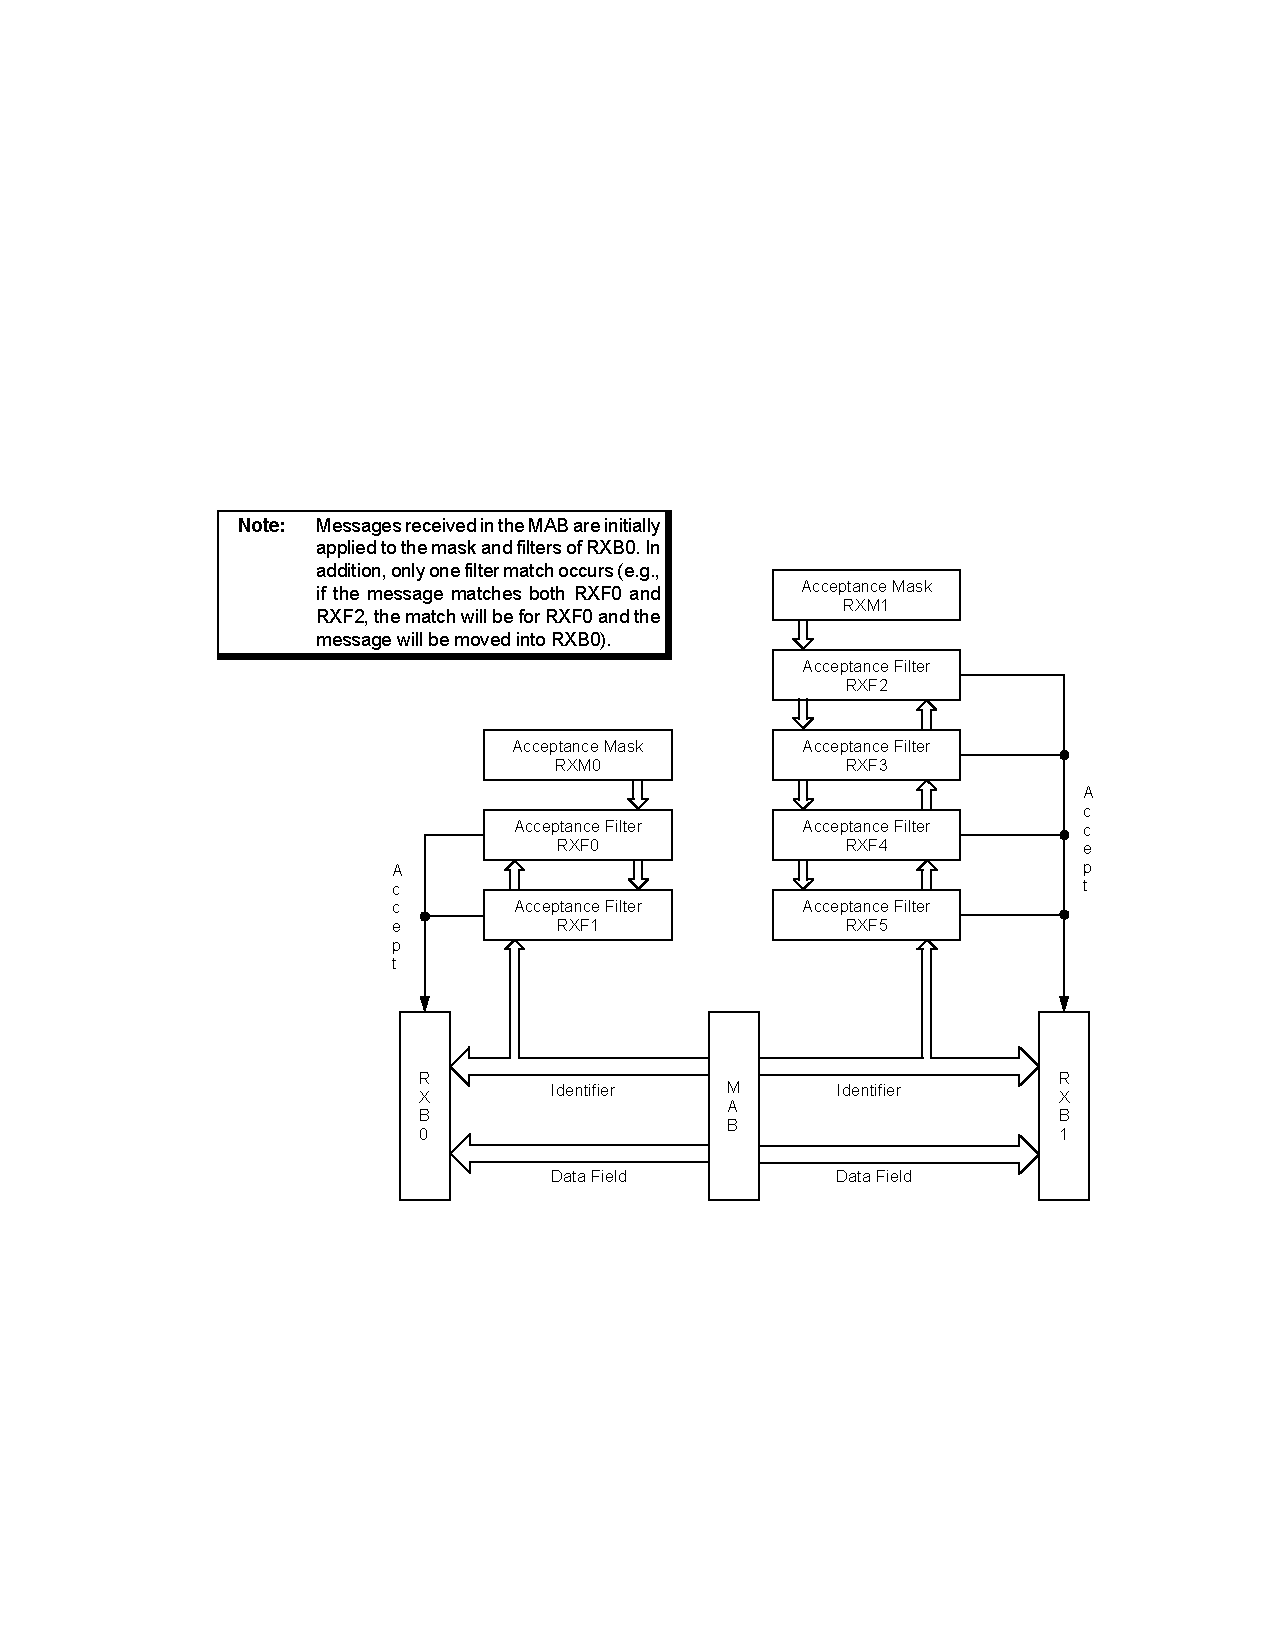
\includegraphics[width=12cm]{mcp2515-filters.pdf}
  \caption{\texttt{MCP2515} acceptance filters (\texttt{DS20001801H}, figure 4.2 page 25)}
  \labelFigure{figureFiltres2515}
\end{figure}








\subsectionLabel{Default behaviour}{defautFilterBehaviour}

The \texttt{can.begin (settings, [] { can.isr () ; })} method sets the \texttt{RXM0} and \texttt{RXM1} registers to $0$, so, the \texttt{MCP2515} receives all CAN bus messages.

More precisely, as \texttt{RXM0} is zero, all messages are received in \texttt{RXB0}. If a new message is received when \texttt{RXB0} is full, the new message is transferred in \texttt{RXB1}. If \texttt{RXB1} is full, the new message is lost.

You can set the \texttt{mRolloverEnable} property of your \texttt{ACAN2515Settings} object to \texttt{false} (it is \texttt{true} by default) to change this default behaviour. When \texttt{mRolloverEnable} is set to \texttt{false}, if a new message is received when \texttt{RXB0} is full, the new message is lost.




\subsectionLabel{Defining filters}{definingFilters}

{\bf Sample sketch: } the \texttt{loopbackUsingFilters} sketch shows how defining filters.

For defining filters, you should:
\begin{itemize}
  \item define the values for the \texttt{RXM0} and \texttt{RXM1} acceptance masks;
  \item submitting an \texttt{ACAN2515AcceptanceFilter} array to the \texttt{ACAN2515::begin} method.
\end{itemize}

The \texttt{ACAN2515AcceptanceFilter} array defines the values that the \texttt{ACAN2515::begin} method sets to the \texttt{RXF$i$} acceptance filter registers.

Four functions are available for managing filters:
\begin{itemize}
  \item \texttt{standard2515Mask} and \texttt{extended2515Mask} functions for defining \texttt{RXM$i$} value;
  \item \texttt{standard2515Filter} and \texttt{extended2515Filter} functions for defining \texttt{RXF$i$} value.
\end{itemize}

\texttt{RXM$i$} and \texttt{RXF$i$} values you handle are \texttt{ACAN2515Mask} class instances, that provides four \texttt{uint8\_t} properties: \texttt{mSIDH}, \texttt{mSIDL}, \texttt{mEID8}, \texttt{mEID0}. They correspond to the \texttt{MCP2515} registers. If you want, you can set directly these properties, without using the above functions. 

{\bf Filter remote and data frames.} The \texttt{MCP2515} filters do not handle the \texttt{RTR} bit: for example, you cannot specify you want to accept data frames and discard remote frames. This should be done by your code.

{\bf Multiple filter matches.} From \texttt{DS20001801H}, section 4.5.4 page 34: \emph{If more than one acceptance filter matches, the FILHITn bits will encode the binary value of the lowest numbered filter that matched. For example, if filters, RXF2 and RXF4, match, the FILHITn bits will be loaded with the value for RXF2. This essentially prioritizes the acceptance filters with a lower numbered filter having higher priority. Messages are compared to filters in ascending order of filter number. This also ensures that the message will only be received into one buffer. This implies that RXB0 has a higher priority than RXB1.}

The \texttt{MCP2515} filters cannot be disabled, so all mask registers can be taken into account during the acceptance of a message. For example, if \texttt{MCP2515} filters are defined with the \texttt{RXM0}, \texttt{RXF0}, \texttt{RXF1} registers, leaving \texttt{RXM1} equal to $0$ provides the transfer to \texttt{RXB1} of all messages discarded by \texttt{RXF0} and \texttt{RXF1}.

For dealing with all situations, the \texttt{ACAN2515::begin} method accepts three prototypes.

\subsubsectionLabel{No filter}{noFilter}
{ \small\begin{lstlisting}[language=c++]
  ACAN2515Settings settings (QUARTZ_FREQUENCY, 125 * 1000) ;
  const uint16_t errorCode = can.begin (settings, [] { can.isr () ; }) ;
\end{lstlisting}}
No filter is provided, \texttt{RXM0} and \texttt{RXM1} are set to $0$, enabling the acceptance of all messages by \texttt{RXB0}.



\subsubsectionLabel{One filter}{oneFilter}

For example:
{ \small\begin{lstlisting}[language=c++]
  ACAN2515Settings settings (QUARTZ_FREQUENCY, 125 * 1000) ;
  const ACAN2515Mask rxm0 = extended2515Mask (0x1FFFFFFF) ;
  const ACAN2515AcceptanceFilter filter [] = {
    {extended2515Filter (0x12345678), receive0} // RXF0
  } ;
  const uint16_t errorCode = can.begin (settings,
                                        [] { can.isr () ; },
                                        rxm0, // Value set to RXM0 register
                                        filter, // The filter array
                                        1) ; // Filter array size
\end{lstlisting}}

Here, one type of message is accepted, extended (data or remote) frames with an identifier equal to \texttt{0x12345678}. This defines explicitly \texttt{RXM0} and \texttt{RXF0}; for disabling acceptance by \texttt{RXF1}, it is set with \texttt{RXF0} value; \texttt{RXM1} is set with \texttt{RXM0} value, and the \texttt{RXF2} to \texttt{RXF5} registers are set with the \texttt{RXF0} value. No message will be accepted by \texttt{RXB1} filters.

The definition of a filter is associated with a call back function -- here \texttt{receive0}. This function is called indirectly when the \texttt{dispatchReceivedMessage} method is called -- see \refSectionPage{UsingDispatchMethod}.








\subsubsectionLabel{Two filters}{twoFilters}

For example:
{ \small\begin{lstlisting}[language=c++]
  ACAN2515Settings settings (QUARTZ_FREQUENCY, 125 * 1000) ;
  const ACAN2515Mask rxm0 = extended2515Mask (0x1FFFFFFF) ;
  const ACAN2515AcceptanceFilter filters [] = {
    {extended2515Filter (0x12345678), receive0}, // RXF0
    {extended2515Filter (0x18765432), receive1}  // RXF1
  } ;
  const uint16_t errorCode = can.begin (settings,
                                        [] { can.isr () ; },
                                        rxm0, // Value set to RXM0 register
                                        filters, // The filter array
                                        2) ; // Filter array size
\end{lstlisting}}

Here, two types of message are accepted, extended (data or remote) frames with an identifier equal to \texttt{0x12345678} or \texttt{0x18765432}. This defines explicitly \texttt{RXM0}, \texttt{RXF0} and \texttt{RXF1}; \texttt{RXM1} is set with \texttt{RXM0} value, and the \texttt{RXF2} to \texttt{RXF5} registers are set with the \texttt{RXF1} value. No message will be accepted by \texttt{RXB1} filters.










\subsubsectionLabel{Three to five filters}{threeToFiveFilters}

For example, with four filters:
{ \small\begin{lstlisting}[language=c++]
  ACAN2515Settings settings (QUARTZ_FREQUENCY, 125 * 1000) ;
  const ACAN2515Mask rxm0 = extended2515Mask (0x1FFFFFFF) ;
  const ACAN2515Mask rxm1 = standard2515Mask (0x7FF, 0, 0) ;
  const ACAN2515AcceptanceFilter filters [] = {
    {extended2515Filter (0x12345678), receive0}, // RXF0
    {extended2515Filter (0x18765432), receive1}, // RXF1
    {standard2515Filter (0x567, 0, 0), receive2},// RXF2
    {standard2515Filter (0x123, 0, 0), receive3} // RXF3
  } ;
  const uint16_t errorCode = can.begin (settings,
                                        [] { can.isr () ; },
                                        rxm0, // Value set to RXM0 register
                                        rxm1, // Value set to RXM1 register
                                        filters, // The filter array
                                        4) ; // Filter array size
\end{lstlisting}}

Four types of message are accepted, extended (data or remote) frames with an identifier equal to \texttt{0x12345678} or \texttt{0x18765432}, and standard (data or remote) frames with an identifier equal to \texttt{0x567} or \texttt{0x123}. The \texttt{RXF4} and \texttt{RXF5} registers are set with the \texttt{RXF3} value.








\subsubsectionLabel{Six filters}{sixFilters}
{ \small\begin{lstlisting}[language=c++]
  ACAN2515Settings settings (QUARTZ_FREQUENCY, 125 * 1000) ;
  const ACAN2515Mask rxm0 = extended2515Mask (0x1FFFFFFF) ;
  const ACAN2515Mask rxm1 = standard2515Mask (0x7FF, 0, 0) ;
  const ACAN2515AcceptanceFilter filters [] = {
    {extended2515Filter (0x12345678), receive0}, // RXF0
    {extended2515Filter (0x18765432), receive1}, // RXF1
    {standard2515Filter (0x567, 0, 0), receive2},// RXF2
    {standard2515Filter (0x123, 0, 0), receive3},// RXF3
    {standard2515Filter (0x777, 0, 0), receive4},// RXF4
    {standard2515Filter (0x3AB, 0, 0), receive5} // RXF5
  } ;
  const uint16_t errorCode = can.begin (settings,
                                        [] { can.isr () ; },
                                        rxm0, // Value set to RXM0 register
                                        rxm1, // Value set to RXM1 register
                                        filters, // The filter array
                                        6) ; // Filter array size
\end{lstlisting}}

Six types of message are accepted, all filter registers are explicitly defined.










\subsection{Extended frames acceptance}

The \texttt{extended2515Mask} and \texttt{extended2515Filter} functions helps you to define extended frame filters. Extended frame filters test extended identifier value.

The acceptance criterion is\footnote{See DS20001801H, section 4.5 \emph{Message Acceptance Filters and Masks}, page 33.}:

\begin{center}
\texttt{acceptance\_mask} {\bf \&} (\texttt{received\_identifier} \texttt{\bf nXOR} \texttt{acceptance\_filter}) == 0
\end{center}
where \& is the bit-wise \emph{and} operator, and \texttt{nXOR} is the \emph{not xor} bit-wise operator.

{\bf Accepting all extended frames.}
{ \small\begin{lstlisting}[language=c++]
  const ACAN2515Mask rxm0 = extended2515Mask (0) ;
\end{lstlisting}}
No extended frame identifier bit is tested, all extended frames are accepted.

{\bf Accepting individual extended frames.}
{ \small\begin{lstlisting}[language=c++]
  const ACAN2515Mask rxm0 = extended2515Mask (0x1FFFFFFF) ;
\end{lstlisting}}
All extended frame identifier bits are tested, only extended frames whose identifiers match the filters are accepted.


{\bf Accepting several identifiers.}
The bits at 0 of the mask correspond to bits that are not tested for acceptance. For example:
{ \small\begin{lstlisting}[language=c++]
  const ACAN2515Mask rxm0 = extended2515Mask (0x1FFFFF0F) ;
\end{lstlisting}}

If you define an acceptance filter by \texttt{extended2515Filter (0x12345608)}, any extended frame with an identifier equal to \texttt{0x123456$x$8} is accepted.












\subsection{Standard frames acceptance}

The \texttt{standard2515Mask} and \texttt{standard2515Filter} functions helps you to define extended frame filters. Standard frame filters test standard identifier value, first and second data byte.

The acceptance criterion is\footnote{See DS20001801H, section 4.5 \emph{Message Acceptance Filters and Masks}, page 33.}:

\begin{center}\small
\texttt{acceptance\_mask} \& (\texttt{(received\_identifier, data\_byte$_0$, data\_byte$_1$)} \texttt{nXOR} \texttt{acceptance\_filter}) == 0
\end{center}
where \& is the bit-wise \emph{and} operator, and \texttt{nXOR} is the \emph{not xor} bit-wise operator.

{\bf Accepting all standard frames, without testing data bytes.}
{ \small\begin{lstlisting}[language=c++]
  const ACAN2515Mask rxm0 = standard2515Mask (0, 0, 0) ;
\end{lstlisting}}

{\bf Accepting individual standard frames, without testing data bytes.}
{ \small\begin{lstlisting}[language=c++]
  const ACAN2515Mask rxm0 = standard2515Mask (0x7FF, 0, 0) ;
\end{lstlisting}}
All standard frame identifier bits are tested, only standard frames whose identifiers match the filters are accepted.


{\bf Accepting several identifiers, without testing data bytes.}
The bits at 0 of the mask correspond to bits that are not tested for acceptance. For example:
{ \small\begin{lstlisting}[language=c++]
  const ACAN2515Mask rxm0 = standard2515Mask (0x70F, 0, 0) ;
\end{lstlisting}}

If you define an acceptance filter by \texttt{standard2515Filter (0x40A, 0, 0)}, any standard frame with an identifier equal to \texttt{0x4$x$A} is accepted.




{\bf Filtering from first data byte.}
The second argument of \texttt{standard2515Mask} specify first data byte filtering. For example:
{ \small\begin{lstlisting}[language=c++]
  const ACAN2515Mask rxm0 = standard2515Mask (0x70F, 0xFF, 0) ;
\end{lstlisting}}

If you define an acceptance filter by \texttt{standard2515Filter (0x40A, 0x54, 0)}, any standard frame with an identifier equal to \texttt{0x4$x$A} and first byte equal to \texttt{0x54} is accepted.

{\bf Empty standard frame.} An empty standard frame (without any data byte) is accepted, the filtering condition on the first data byte is ignored (see \texttt{loopbackFilterDataByte} sample sketch).









\sectionLabel{The \texttt{dispatchReceivedMessage} method}{UsingDispatchMethod}

{\bf Sample sketch: } the \texttt{loopbackUsingFilters} shows how using the \texttt{dispatchReceivedMessage} method.

Instead of calling the \texttt{receive} method, call the \texttt{dispatchReceivedMessage} method in your \texttt{loop} function. It calls the call back function associated with the matching filter.

If you have not defined any filter, do not use this function, call the \texttt{receive} method.


{ \small\begin{lstlisting}[language=c++]
void loop () {
  can.dispatchReceivedMessage () ; // Do not use can.receive any more
  ...
}
\end{lstlisting}}

The \texttt{dispatchReceivedMessage} method handles one message at a time. More precisely:
\begin{itemize}
  \item if it returns \texttt{false}, the driver receive buffer was empty;
  \item if it returns \texttt{true}, the driver receive buffer was not empty, one message has been removed and dispatched.
\end{itemize}

So, the return value can used for emptying and dispatching all received messages:
{ \small\begin{lstlisting}[language=c++]
void loop () {
  while (can.dispatchReceivedMessage ()) {
  }
  ...
}
\end{lstlisting}}

If a filter definition does not name a call back function, the corresponding messages are lost.

The \texttt{dispatchReceivedMessage} method has an optional argument -- \texttt{NULL} by default: a function name. This function is called for every message that pass the receive filters, with an argument equal to the matching filter index:

{ \small\begin{lstlisting}[language=c++]
void filterMatchFunction (const uint8_t inFilterIndex) {
  ...
}

void loop () {
  can.dispatchReceivedMessage (filterMatchFunction) ;
  ...
}
\end{lstlisting}}

You can use this function for maintaining statistics about receiver filter matches.


\sectionLabel{The \texttt{ACAN2515::begin} method reference}{beginMethodReference}

\subsection{The \texttt{ACAN2515::begin} method prototypes}

There are three \texttt{begin} method prototypes:
{ \small\begin{lstlisting}[language=c++]
uint16_t ACAN2515::begin (const ACAN2515Settings & inSettings,
                          void (* inInterruptServiceRoutine) (void)) ;
\end{lstlisting}}

{ \small\begin{lstlisting}[language=c++]
uint16_t ACAN2515::begin (const ACAN2515Settings & inSettings,
                          void (* inInterruptServiceRoutine) (void),
                          const ACAN2515Mask inRXM0,
                          const ACAN2515AcceptanceFilter inAcceptanceFilters [],
                          const uint32_t inAcceptanceFilterCount) ;
\end{lstlisting}}

{ \small\begin{lstlisting}[language=c++]
uint16_t ACAN2515::begin (const ACAN2515Settings & inSettings,
                          void (* inInterruptServiceRoutine) (void),
                          const ACAN2515Mask inRXM0,
                          const ACAN2515Mask inRXM1,
                          const ACAN2515AcceptanceFilter inAcceptanceFilters [],
                          const uint32_t inAcceptanceFilterCount) ;
\end{lstlisting}}



\subsectionLabel{Defining explicitly the interrupt service routine}{isrExplicit}

In this document, the \emph{interrupt service routine} is defined by a lambda expression:
{ \small\begin{lstlisting}[language=c++]
  const uint16_t errorCode = can.begin (settings, [] { can.isr () ; }) ;
\end{lstlisting}}

Instead of a lambda expression, you are free to define the \emph{interrupt service routine} as a function:
{ \small\begin{lstlisting}[language=c++]
void canISR () {
  can.isr () ;
}
\end{lstlisting}}

And you pass \texttt{canISR} as argument to the \texttt{begin} method:
{ \small\begin{lstlisting}[language=c++]
  const uint16_t errorCode = can.begin (settings, canISR) ;
\end{lstlisting}}


\subsectionLabel{The error code}{errorCodeMethodBegin}

The \texttt{ACAN2515::begin} and \texttt{ACAN2515::setFiltersOnTheFly} methods return an error code. The value \texttt{0} denotes no error. Otherwise, you consider every bit as an error flag, as described in \refTableau{beginErrorCode}. An error code could report several errors. The \texttt{ACAN2515} class defines static constants for naming errors.


\begin{table}[!ht]
  \small
  \onehalfspacing
  \centering
  \begin{tabular}{rll}
    \textbf{Bit} & \textbf{Static constant Name}         & \textbf{Link}\\
    \texttt{0} & \texttt{kNoMCP2515} & \refSubsubsectionPage{kNoMCP2515}\\
    \texttt{1} & \texttt{kTooFarFromDesiredBitRate} & \refSubsubsectionPage{kTooFarFromDesiredBitRate} \\
    \texttt{2} & \texttt{kInconsistentBitRateSettings} & \refSubsubsectionPage{kInconsistentBitRateSettings} \\
    \texttt{3} & \texttt{kINTPinIsNotAnInterrupt} & \refSubsubsectionPage{kINTPinIsNotAnInterrupt} \\
    \texttt{4} & \texttt{kISRIsNull}  & \refSubsubsectionPage{kISRIsNull} \\
    \texttt{5} & \texttt{kRequestedModeTimeOut} & \refSubsubsectionPage{kRequestedModeTimeOut}\\
    \texttt{6} & \texttt{kAcceptanceFilterArrayIsNULL} & \refSubsubsectionPage{kAcceptanceFilterArrayIsNULL} \\
    \texttt{7} & \texttt{kOneFilterMaskRequiresOneOrTwoAcceptanceFilters} & \refSubsubsectionPage{kOneFilterMaskRequiresOneOrTwoAcceptanceFilters} \\
    \texttt{8} & \texttt{kTwoFilterMasksRequireThreeToSixAcceptanceFilters} & \refSubsubsectionPage{kTwoFilterMasksRequireThreeToSixAcceptanceFilters}\\
    \texttt{9} & \texttt{kCannotAllocateReceiveBuffer} & \refSubsubsectionPage{kCannotAllocateReceiveBuffer}\\
    \texttt{10} & \texttt{kCannotAllocateTransmitBuffer0} & \refSubsubsectionPage{kCannotAllocateTransmitBuffer0}\\
    \texttt{11} & \texttt{kCannotAllocateTransmitBuffer1} & \refSubsubsectionPage{kCannotAllocateTransmitBuffer1}\\
    \texttt{12} & \texttt{kCannotAllocateTransmitBuffer2} & \refSubsubsectionPage{kCannotAllocateTransmitBuffer2}\\
    \texttt{13} & \texttt{kISRNotNullAndNoIntPin}         & \refSubsubsectionPage{kISRNotNullAndNoIntPin} \\
  \end{tabular}
  \caption{The \texttt{ACAN2515::begin} method error code bits}
  \labelTableau{beginErrorCode}
\end{table}




\subsubsectionLabel{\texttt{kNoMCP2515}}{kNoMCP2515}

The \texttt{ACAN2515::begin} method checks accessibility by writing and reading back the \texttt{CNF1\_REGISTER} first with the \texttt{0x55} value, then with the \texttt{0xAA} value. This error is raised when the read value is different from the written one. It means that the \texttt{MCP2515} cannot be accessed via SPI. 

\subsubsectionLabel{\texttt{kTooFarFromDesiredBitRate}}{kTooFarFromDesiredBitRate}

This error occurs when the \texttt{mBitRateClosedToDesiredRate} property of the \texttt{settings} object is \texttt{false}. This means that the \texttt{ACAN2515Settings} constructor cannot compute a CAN bit configuration close enough to the desired bit rate. For example:

{ \small\begin{lstlisting}[language=c++]
void setup () {
  ACAN2515Settings settings (QUARTZ_FREQUENCY, 1) ; // 1 bit/s !!!
  // Here, settings.mBitRateClosedToDesiredRate is false
  const uint16_t errorCode = can.begin (settings, [] { can.isr () ; }) ;
  // Here, errorCode contains ACAN2515::kCANBitConfigurationTooFarFromDesiredBitRate
}
\end{lstlisting}}




\subsubsectionLabel{\texttt{kInconsistentBitRateSettings}}{kInconsistentBitRateSettings}

The \texttt{ACAN2515Settings} constructor always returns consistent bit rate settings -- even if the settings provide a bit rate too far away the desired bit rate. So this error occurs only when you have changed the CAN bit properties (\texttt{mBitRatePrescaler}, \texttt{mPropagationSegment}, \texttt{mPhaseSegment1}, \texttt{mPhaseSegment2}, \texttt{mSJW}), and one or more resulting values are inconsistent. See \refSubsectionPage{CANBitSettingConsistency}.











\subsubsectionLabel{\texttt{kINTPinIsNotAnInterrupt}}{kINTPinIsNotAnInterrupt}

The pin you provide for handling the \texttt{MCP2515} interrupt has no interrupt capability.

\subsubsectionLabel{\texttt{kISRIsNull}}{kISRIsNull}

The interrupt service routine argument is \texttt{NULL}, you should provide a valid function.


\subsubsectionLabel{\texttt{kRequestedModeTimeOut}}{kRequestedModeTimeOut}

During configuration by the \texttt{ACAN2515::begin} method, the  \texttt{MCP2515} is in the \emph{configuration} mode. At this end of this process, the mode specified by the \texttt{inSettings.mRequestedMode} value is requested. The switch to this mode is not immediate, a register is repetitively read for checking the switch is done. This error is raised if the switch is not completed within a delay between 1 ms and 2 ms.






\subsubsectionLabel{\texttt{kAcceptanceFilterArrayIsNULL}}{kAcceptanceFilterArrayIsNULL}

The \texttt{ACAN2515::begin} method you have called names the \texttt{inAcceptanceFilters} argument, but it is \texttt{NULL}.






\subsubsectionLabel{\texttt{kOneFilterMaskRequiresOneOrTwoAcceptanceFilters}}{kOneFilterMaskRequiresOneOrTwoAcceptanceFilters}

The \texttt{ACAN2515::begin} method you have called names the \texttt{inRXM0} argument (but not \texttt{inRXM1}), you should provide the value $1$ or $2$ to the \texttt{inAcceptanceFilterCount} argument.







\subsubsectionLabel{\texttt{kTwoFilterMasksRequireThreeToSixAcceptanceFilters}}{kTwoFilterMasksRequireThreeToSixAcceptanceFilters}

The \texttt{ACAN2515::begin} method you have called names the \texttt{inRXM0} and the the \texttt{inRXM1} arguments, you should provide the value $3$ to $6$ to the \texttt{inAcceptanceFilterCount} argument.



\subsubsectionLabel{\texttt{kCannotAllocateReceiveBuffer}}{kCannotAllocateReceiveBuffer}

There is not enough RAM left to allocate the receive buffer. Try to reduce its size (see \refSubsectionPage{driverReceiveBufferSize}), and / or to reduce transmit buffer sizes (\refSubsectionPage{driverTransmitBufferSize}).

Note a memory overflow is not always detected properly: dynamic allocation can be successful, leaving too little memory available for a later allocation of automatic variables, which can cause a crash.



\subsubsectionLabel{\texttt{kCannotAllocateTransmitBuffer0}}{kCannotAllocateTransmitBuffer0}

There is not enough RAM left to allocate the transmit buffer 0. Try to reduce its size (see \refSubsectionPage{driverTransmitBufferSize}), and / or to reduce receive buffer size (\refSubsectionPage{driverReceiveBufferSize}).

Note a memory overflow is not always detected properly: dynamic allocation can be successful, leaving too little memory available for a later allocation of automatic variables, which can cause a crash.



\subsubsectionLabel{\texttt{kCannotAllocateTransmitBuffer1}}{kCannotAllocateTransmitBuffer1}

There is not enough RAM left to allocate the transmit buffer 1. Try to reduce its size (see \refSubsectionPage{driverTransmitBufferSize}), and / or to reduce receive buffer size (\refSubsectionPage{driverReceiveBufferSize}).

Note a memory overflow is not always detected properly: dynamic allocation can be successful, leaving too little memory available for a later allocation of automatic variables, which can cause a crash.




\subsubsectionLabel{\texttt{kCannotAllocateTransmitBuffer2}}{kCannotAllocateTransmitBuffer2}

There is not enough RAM left to allocate the transmit buffer 2. Try to reduce its size (see \refSubsectionPage{driverTransmitBufferSize}), and / or to reduce receive buffer size (\refSubsectionPage{driverReceiveBufferSize}).

Note a memory overflow is not always detected properly: dynamic allocation can be successful, leaving too little memory available for a later allocation of automatic variables, which can cause a crash.





\subsubsectionLabel{\texttt{kISRNotNullAndNoIntPin}}{kISRNotNullAndNoIntPin}

This error occurs when you have no \texttt{INT} pin, and a not-null interrupt service routine: 
{ \small\begin{lstlisting}[language=c++]
ACAN2515 can (MCP2515_CS, SPI, 255) ; // Last argument is 255 -> no interrupt pin

void setup () {
  ...
  const uint16_t errorCode = can.begin (settings, [] { can.isr () ; }) ; // ISR is not null
  ...
}
\end{lstlisting}}

Interrupt service routine should be \texttt{NULL} if no \texttt{INT} pin is defined:
{ \small\begin{lstlisting}[language=c++]
ACAN2515 can (MCP2515_CS, SPI, 255) ; // Last argument is 255 -> no interrupt pin

void setup () {
  ...
  const uint16_t errorCode = can.begin (settings, NULL) ; // Ok, ISR is null
  ...
}
\end{lstlisting}}

See the \texttt{LoopBackDemoTeensy3x-no-int} and \texttt{LoopBackDemoESP32-no-int} sketches.













\sectionLabel{The \texttt{ACAN2515::changeModeOnTheFly} function}{changeModeOnTheFlyFunction}

{\bf Note. } Available in release 2.0.0 and later.

{ \small\begin{lstlisting}[language=c++]
uint16_t ACAN2515::
  changeModeOnTheFly (const ACAN2515Settings::RequestedMode inRequestedMode);
\end{lstlisting}}

After the library has been initialized by a call to \texttt{ACAN2515::begin} that returns no errors (i.e. zero), you can call this function to change modes on the fly. It returns \texttt{0} if it succeeds. If it fails, it returns the \texttt{kRequestedModeTimeOut} error, indicating that the requested mode cannot be reached within 2 ms (see \refSubsubsectionPage{kRequestedModeTimeOut}).

{\bf Note. } The function preserves contents of the bits 0 ... 4 of the \texttt{CANCTRL} register.
















\sectionLabel{The \texttt{ACAN2515::setFiltersOnTheFly} functions}{setFiltersOnTheFlyFunction}

{\bf Note. } Available in release 2.0.0 and later.

There are three \texttt{setFiltersOnTheFly} method prototypes:

{ \small\begin{lstlisting}[language=c++]
uint16_t ACAN2515::setFiltersOnTheFly (void);

uint16_t ACAN2515::
  setFiltersOnTheFly (const ACAN2515Mask inRXM0,
                      const ACAN2515AcceptanceFilter inAcceptanceFilters [],
                      const uint8_t inAcceptanceFilterCount) ;

uint16_t ACAN2515::
  setFiltersOnTheFly (const ACAN2515Mask inRXM0,
                      const ACAN2515Mask inRXM1,
                      const ACAN2515AcceptanceFilter inAcceptanceFilters [],
                      const uint8_t inAcceptanceFilterCount) ;
\end{lstlisting}}

After the library has been initialized by a call to \texttt{ACAN2515::begin} that returns no errors (i.e. zero), you can call this function to change filters on the fly. It returns \texttt{0} if it succeeds. If it fails, it returns a non zero \texttt{uint16\_t} value (see \refSubsectionPage{errorCodeMethodBegin}).

The three \texttt{setFiltersOnTheFly} method prototypes correspond to the three \texttt{begin} method prototypes, they handle filter definition in the same way (see \refSubsectionPage{definingFilters}).

\subsection{No filter}
{ \small\begin{lstlisting}[language=c++]
  const uint16_t errorCode = can.setFiltersOnTheFly () ;
\end{lstlisting}}
No filter is provided, \texttt{RXM0} and \texttt{RXM1} are set to $0$, enabling the acceptance of all messages by \texttt{RXB0}.



\subsection{One filter}

For example:
{ \small\begin{lstlisting}[language=c++]
  const ACAN2515Mask rxm0 = extended2515Mask (0x1FFFFFFF) ;
  const ACAN2515AcceptanceFilter filter [] = {
    {extended2515Filter (0x12345678), receive0} // RXF0
  } ;
  const uint16_t errorCode = can.setFiltersOnTheFly (
                                        rxm0, // Value set to RXM0 register
                                        filter, // The filter array
                                        1) ; // Filter array size
\end{lstlisting}}

Here, one type of message is accepted, extended (data or remote) frames with an identifier equal to \texttt{0x12345678}. This defines explicitly \texttt{RXM0} and \texttt{RXF0}; for disabling acceptance by \texttt{RXF1}, it is set with \texttt{RXF0} value; \texttt{RXM1} is set with \texttt{RXM0} value, and the \texttt{RXF2} to \texttt{RXF5} registers are set with the \texttt{RXF0} value. No message will be accepted by \texttt{RXB1} filters.

The definition of a filter is associated with a call back function -- here \texttt{receive0}. This function is called indirectly when the \texttt{dispatchReceivedMessage} method is called -- see \refSectionPage{UsingDispatchMethod}.








\subsection{Two filters}

For example:
{ \small\begin{lstlisting}[language=c++]
  const ACAN2515Mask rxm0 = extended2515Mask (0x1FFFFFFF) ;
  const ACAN2515AcceptanceFilter filters [] = {
    {extended2515Filter (0x12345678), receive0}, // RXF0
    {extended2515Filter (0x18765432), receive1}  // RXF1
  } ;
  const uint16_t errorCode = can.setFiltersOnTheFly (
                                        rxm0, // Value set to RXM0 register
                                        filters, // The filter array
                                        2) ; // Filter array size
\end{lstlisting}}

Here, two types of message are accepted, extended (data or remote) frames with an identifier equal to \texttt{0x12345678} or \texttt{0x18765432}. This defines explicitly \texttt{RXM0}, \texttt{RXF0} and \texttt{RXF1}; \texttt{RXM1} is set with \texttt{RXM0} value, and the \texttt{RXF2} to \texttt{RXF5} registers are set with the \texttt{RXF1} value. No message will be accepted by \texttt{RXB1} filters.










\subsection{Three to five filters}

For example, with four filters:
{ \small\begin{lstlisting}[language=c++]
  const ACAN2515Mask rxm0 = extended2515Mask (0x1FFFFFFF) ;
  const ACAN2515Mask rxm1 = standard2515Mask (0x7FF, 0, 0) ;
  const ACAN2515AcceptanceFilter filters [] = {
    {extended2515Filter (0x12345678), receive0}, // RXF0
    {extended2515Filter (0x18765432), receive1}, // RXF1
    {standard2515Filter (0x567, 0, 0), receive2},// RXF2
    {standard2515Filter (0x123, 0, 0), receive3} // RXF3
  } ;
  const uint16_t errorCode = can.setFiltersOnTheFly (
                                        rxm0, // Value set to RXM0 register
                                        rxm1, // Value set to RXM1 register
                                        filters, // The filter array
                                        4) ; // Filter array size
\end{lstlisting}}

Four types of message are accepted, extended (data or remote) frames with an identifier equal to \texttt{0x12345678} or \texttt{0x18765432}, and standard (data or remote) frames with an identifier equal to \texttt{0x567} or \texttt{0x123}. The \texttt{RXF4} and \texttt{RXF5} registers are set with the \texttt{RXF3} value.








\subsection{Six filters}
{ \small\begin{lstlisting}[language=c++]
  const ACAN2515Mask rxm0 = extended2515Mask (0x1FFFFFFF) ;
  const ACAN2515Mask rxm1 = standard2515Mask (0x7FF, 0, 0) ;
  const ACAN2515AcceptanceFilter filters [] = {
    {extended2515Filter (0x12345678), receive0}, // RXF0
    {extended2515Filter (0x18765432), receive1}, // RXF1
    {standard2515Filter (0x567, 0, 0), receive2},// RXF2
    {standard2515Filter (0x123, 0, 0), receive3},// RXF3
    {standard2515Filter (0x777, 0, 0), receive4},// RXF4
    {standard2515Filter (0x3AB, 0, 0), receive5} // RXF5
  } ;
  const uint16_t errorCode = can.setFiltersOnTheFly (
                                        rxm0, // Value set to RXM0 register
                                        rxm1, // Value set to RXM1 register
                                        filters, // The filter array
                                        6) ; // Filter array size
\end{lstlisting}}

Six types of message are accepted, all filter registers are explicitly defined.














\sectionLabel{The \texttt{ACAN2515::end} method}{endFunction}

{\bf Note. } Available in release 2.0.0 and later.

{ \small\begin{lstlisting}[language=c++]
void ACAN2515::end (void) ;
\end{lstlisting}}

After the library has been initialized by a call to \texttt{ACAN2515::begin} that returns no errors (i.e. zero), you can call this function to reset the \texttt{MCP2515}. It also frees the driver transmit and receive buffers, and, if interrupt pin is actually used (i.e. its number is different from 255), detach interrupt from interrupt pin.














\sectionLabel{The \texttt{ACAN2515} instance usage}{canInstanceUsage}

The \texttt{ACAN2515} instance usage graph is given in \refFigure{}{canInstanceUsage}.



\begin{figure}[!ht]
%  \small
  \centering
  \begin{tikzpicture}[line cap=round, line join=round, >=stealth]
  %--- Nœuds
    \node[draw] (NE) at (0, 2) {\bf Non-existent};
    \node[draw] (IN) at (0,0) {\bf Initialized};
    \node[draw, diamond] (TE) at (0,-2) {\small Ok?};
    \node[draw] (OP) at (0,-4) {\bf Operational};
    \node[draw, diamond] (TO) at (0,-6) {\small Ok?};
    \node[draw] (IV) at (0,-8) {\bf Invalid};
  %--- Flèches
    \draw[->] (NE) to[bend right] node[pos=0.5, left] {(1) Constructor} (IN);
    \draw[->] (IN) to[bend right] node[pos=0.5, right] {(10) Destructor} (NE);
    \draw[->] (IN) -- node[pos=0.5, left] {(2) \texttt{begin}} (TE);
    \draw[->] (TE) -- node[pos=0.5, left] {(3) No error} (OP);
    \draw[->,color=red] (TE.east) to[bend right,out=-90] node[pos=0.5, right] {\textcolor{red}{(4) Error}} (IN.south east);
    \draw[->] (OP.east) to[bend right,out=-90,in=-90] node[pos=0.5, right] {(5) \texttt{end}} (IN.east);
    \draw[->] (OP) -- node[pos=0.5, left] {(6) \texttt{xxxOnTheFly}} (TO);
    \draw[->] (TO.east) to[bend right,out=-90] node[pos=0.5, right] {(7) No error} (OP.south east);
    \draw[->,color=red] (TO) -- node[pos=0.5, right] {\textcolor{red}{(8) Error}} (IV);
    \draw[->] (IV.east) to[bend right,out=-90,in=-90] node[pos=0.5, right] {(9) \texttt{end}} (IN.east);
  %---
  \end{tikzpicture}
  \caption{ACAN2515 instance usage}
  \labelFigure{canInstanceUsage}
\end{figure}

The state are:
\begin{itemize}
  \item {\bf Non-existent}, the \texttt{can} object does not exist or is not initialized;
  \item {\bf Initialized}, the \texttt{can} object is initialized;
  \item {\bf Operational}, the \texttt{can} object is operational, you can use it from communication (functions \texttt{tryToSend}, \texttt{available}, \texttt{receive}, \texttt{dispatchReceivedMessage}, ...); note the actual possibilities depends from the requested mode: in \texttt{ListenOnlyMode} messages cannot be sent; in \texttt{SleepMode} no communication is handled.
  \item {\bf Invalid}, a call of \texttt{changeModeOnTheFly} or  \texttt{setFiltersOnTheFly} has returned an error, the \texttt{can} object should be reseted by a call to the \texttt{endø} function. 
\end{itemize}

In many situations, only transitions (1), (2) and (3) are performed.

{ \small\begin{lstlisting}[language=c++]
// Here, the can object does not exist ("Non-existent" state)
ACAN2515 can (...) ; // Performs (1)
// Here, can object is in "Initialized" state

void setup () {
  ...
  const uint16_t errorCode = can.begin (...) ; // Performs (2) (3) or (2) (4)
  // if errorCode is 0, can object is in "Operational" state;
  // otherwise, it remains in "Initialized" state.
  ...
}
\end{lstlisting}}









\sectionLabel{\texttt{ACAN2515Settings} class reference}{ACAN2515SettingsRef}

{\bf Note. } The \texttt{ACAN2515Settings} class is not Arduino specific. You can compile it on your desktop computer with your favorite C++ compiler. In the \url{https://github.com/pierremolinaro/acan2515-dev} GitHub repository, a command line tool is defined for exploring all CAN bit rates from 1 bit/s and 20 Mbit/s for a 16 MHz quartz: 63810 bit rates are valid, and 29 are exact. It also checks that computed CAN bit decompositions are all consistent, even if they are too far from the desired baud rate.



\subsectionLabel{First \texttt{ACAN2515Settings} constructor: computation of the CAN bit settings}{CANbitSettings}

The constructor of the \texttt{ACAN2515Settings} has two mandatory arguments: the quartz frequency, and the desired bit rate. It tries to compute the CAN bit settings for this bit rate. If it succeeds, the constructed object has its \texttt{mBitRateClosedToDesiredRate} property set to \texttt{true}, otherwise it is set to \texttt{false}. For example:
{ \small\begin{lstlisting}[language=c++]
const uint32_t QUARTZ_FREQUENCY = 16 * 1000 * 1000 ; // 16 MHz
void setup () {
  ACAN2515Settings settings (QUARTZ_FREQUENCY, 1 * 1000 * 1000) ; // 1 Mbit/s
  // Here, settings.mBitRateClosedToDesiredRate is true
  ...
}
\end{lstlisting}}

Of course, with a 16 MHz quartz, CAN bit computation always succeeds for classical bit rates: 1 Mbit/s, 500 kbit/s, 250 kbit/s, 125 kbit/s. But CAN bit computation can also succeed for some unusual bit rates, as 727 kbit/s. You can check the result by computing actual bit rate, and the distance from the desired bit rate:
{ \small\begin{lstlisting}[language=c++]
const uint32_t QUARTZ_FREQUENCY = 16 * 1000 * 1000 ; // 16 MHz
void setup () {
  ...
  ACAN2515Settings settings (QUARTZ_FREQUENCY, 727 * 1000) ; // 727 kbit/s
  Serial.print ("mBitRateClosedToDesiredRate: ") ;
  Serial.println (settings.mBitRateClosedToDesiredRate) ; // 1 (--> is true)
  Serial.print ("actual bit rate: ") ;
  Serial.println (settings.actualBitRate ()) ; //  727272 bit/s
  Serial.print ("distance: ") ;
  Serial.println (settings.ppmFromDesiredBitRate ()) ; // 375 ppm
  ...
}
\end{lstlisting}}

The actual bit rate is 727,272 bit/s, and its distance from desired bit rate is 375 ppm. "ppm" stands for "part-per-million", and $1~\texttt{ppm} = 10^{-6}$. In other words, $10,000~\texttt{ppm}=1\%$.


By default, a desired bit rate is accepted if the distance from the computed actual bit rate is lower or equal to $1,000~\texttt{ppm} = 0.1~\%$. You can change this default value by adding your own value as third argument of \texttt{ACAN2515Settings} constructor:
{ \small\begin{lstlisting}[language=c++]
const uint32_t QUARTZ_FREQUENCY = 16 * 1000 * 1000 ; // 16 MHz
void setup () {
  ...
  ACAN2515Settings settings (QUARTZ_FREQUENCY, 727 * 1000, 100) ;
  Serial.print ("mBitRateClosedToDesiredRate: ") ;
  Serial.println (settings.mBitRateClosedToDesiredRate) ; // 0 (--> is false)
  Serial.print ("actual bit rate: ") ;
  Serial.println (settings.actualBitRate ()) ; //  727272 bit/s
  Serial.print ("distance: ") ;
  Serial.println (settings.ppmFromDesiredBitRate ()) ; // 375 ppm
  ...
}
\end{lstlisting}}

The third argument does not change the CAN bit computation, it only changes the acceptance test for setting the \texttt{mBitRateClosedToDesiredRate} property. For example, you can specify that you want the computed actual bit to be exactly the desired bit rate:
{ \small\begin{lstlisting}[language=c++]
const uint32_t QUARTZ_FREQUENCY = 16 * 1000 * 1000 ; // 16 MHz
void setup () {
  ...
  ACAN2515Settings settings (QUARTZ_FREQUENCY, 500 * 1000, 0) ; // Max distance is 0 ppm
  Serial.print ("mBitRateClosedToDesiredRate: ") ;
  Serial.println (settings.mBitRateClosedToDesiredRate) ; // 1 (--> is true)
  Serial.print ("actual bit rate: ") ;
  Serial.println (settings.actualBitRate ()) ; //  500,000 bit/s
  Serial.print ("distance: ") ;
  Serial.println (settings.ppmFromDesiredBitRate ()) ; // 0 ppm
  ...
}
\end{lstlisting}}


In any way, the bit rate computation always gives a consistent result, resulting an actual bit rate closest from the desired bit rate. For example:
{ \small\begin{lstlisting}[language=c++]
const uint32_t QUARTZ_FREQUENCY = 16 * 1000 * 1000 ; // 16 MHz
void setup () {
  ...
  ACAN2515Settings settings (QUARTZ_FREQUENCY, 440 * 1000) ; // 440 kbit/s 
  Serial.print ("mBitRateClosedToDesiredRate: ") ;
  Serial.println (settings.mBitRateClosedToDesiredRate) ; // 0 (--> is false)
  Serial.print ("actual bit rate: ") ;
  Serial.println (settings.actualBitRate ()) ; //  444,444 bit/s
  Serial.print ("distance: ") ;
  Serial.println (settings.ppmFromDesiredBitRate ()) ; // 10,100 ppm
  ...
}
\end{lstlisting}}

You can get the details of the CAN bit decomposition. For example:

{ \small\begin{lstlisting}[language=c++]
const uint32_t QUARTZ_FREQUENCY = 16 * 1000 * 1000 ; // 16 MHz
void setup () {
  ...
  ACAN2515Settings settings (QUARTZ_FREQUENCY, 440 * 1000) ; // 440 kbit/s 
  Serial.print ("mBitRateClosedToDesiredRate: ") ;
  Serial.println (settings.mBitRateClosedToDesiredRate) ; // 0 (--> is false)
  Serial.print ("actual bit rate: ") ;
  Serial.println (settings.actualBitRate ()) ; //  444,444 bit/s
  Serial.print ("distance: ") ;
  Serial.println (settings.ppmFromDesiredBitRate ()) ; // 10,100 ppm
  Serial.print ("Bit rate prescaler: ") ;
  Serial.println (settings.mBitRatePrescaler) ; // BRP = 1
  Serial.print ("Propagation segment: ") ;
  Serial.println (settings.mPropagationSegment) ; // PropSeg = 6
  Serial.print ("Phase segment 1: ") ;
  Serial.println (settings.mPhaseSegment1) ; // PS1 = 5
  Serial.print ("Phase segment 2: ") ;
  Serial.println (settings.mPhaseSegment2) ; // PS2 = 6
  Serial.print ("Resynchronization Jump Width: ") ;
  Serial.println (settings.mSJW) ; // SJW = 4
  Serial.print ("Triple Sampling: ") ;
  Serial.println (settings.mTripleSampling) ; // 0, meaning single sampling
  Serial.print ("Sample Point: ") ;
  Serial.println (settings.samplePointFromBitStart ()) ; // 68, meaning 68%
  Serial.print ("Consistency: ") ;
  Serial.println (settings.CANBitSettingConsistency ()) ; // 0, meaning Ok
  ...
}
\end{lstlisting}}

The \texttt{samplePointFromBitStart} method returns sample point, expressed in per-cent of the bit duration from the beginning of the bit.


Note the computation may calculate a bit decomposition too far from the desired bit rate, but it is always consistent. You can check this by calling the \texttt{CANBitSettingConsistency} method.

You can change the property values for adapting to the particularities of your CAN network propagation time. By example, you can increment the \texttt{mPhaseSegment1} value, and decrement the \texttt{mPhaseSegment2} value in order to sample the \texttt{CAN Rx} pin later.

{ \small\begin{lstlisting}[language=c++]
const uint32_t QUARTZ_FREQUENCY = 16 * 1000 * 1000 ; // 16 MHz
void setup () {
  ...
  ACAN2515Settings settings (QUARTZ_FREQUENCY, 500 * 1000) ; // 500 kbit/s
  Serial.print ("mBitRateClosedToDesiredRate: ") ;
  Serial.println (settings.mBitRateClosedToDesiredRate) ; // 1 (--> is true)
  settings.mPhaseSegment1 ++ ; // 5 -> 6: safe, 1 <= PS1 <= 8
  settings.mPhaseSegment2 -- ; // 5 -> 4: safe, 2 <= PS2 <= 8 and SJW <= PS2
  Serial.print ("Sample Point: ") ;
  Serial.println (settings.samplePointFromBitStart ()) ; // 75, meaning 75%
  Serial.print ("actual bit rate: ") ;
  Serial.println (settings.actualBitRate ()) ; // 500000: ok, bit rate did not change
  Serial.print ("Consistency: ") ;
  Serial.println (settings.CANBitSettingConsistency ()) ; // 0, meaning Ok
  ...
}
\end{lstlisting}}

Be aware to always respect CAN bit timing consistency! The constraints are:

\begin{align*}
1 & \leqslant \texttt{mBitRatePrescaler} \leqslant 64 \\
1 & \leqslant \texttt{mSJW} \leqslant 4 \\
1 & \leqslant \texttt{mPropagationSegment} \leqslant 8 \\
\text{Single sampling: }1 & \leqslant \texttt{mPhaseSegment1} \leqslant 8\\
\text{Triple sampling: }2 & \leqslant \texttt{mPhaseSegment1} \leqslant 8\\
2 & \leqslant \texttt{mPhaseSegment2} \leqslant 8 \\
\texttt{mSJW} &<\texttt{mPhaseSegment2}\\
\texttt{mPhaseSegment2} & \leqslant \texttt{mPropagationSegment} + \texttt{mPhaseSegment1}
\end{align*}

Resulting actual bit rate is given by:
{\small
\begin{align*}
\text{Actual bit rate} & = \frac{QuartzFrequency~/~2}{\texttt{mBitRatePrescaler} \cdot (1 + \texttt{mPropagationSegment} + \texttt{mPhaseSegment1} + \texttt{mPhaseSegment2})}
\end{align*}
}

And sampling points (in per-cent unit) are given by:
{\small
\begin{align*}
\text{Sampling point {\it(single sampling)}} & = 100 \cdot \frac{1 + \texttt{mPropagationSegment} + \texttt{mPhaseSegment1}}{1 + \texttt{mPropagationSegment} + \texttt{mPhaseSegment1} + \texttt{mPhaseSegment2}}  \\
  & \\
\text{Sampling first point {\it(triple sampling)}} & = 100 \cdot \frac{\texttt{mPropagationSegment} + \texttt{mPhaseSegment1}}{1 + \texttt{mPropagationSegment} + \texttt{mPhaseSegment1} + \texttt{mPhaseSegment2}}
\end{align*}
}




\subsectionLabel{Second \texttt{ACAN2515Settings} constructor: explicit CAN bit settings}{explicitCANbitSettings}

{\bf New in release 1.0.4.} This \texttt{ACAN2515Settings} constructor defines explicitly CAN bit settings. For example, see the \texttt{LoopBackDemoBitRateSettings} sketch~:
{ \small\begin{lstlisting}[language=c++]
const uint32_t QUARTZ_FREQUENCY = 16 * 1000 * 1000 ; // 16 MHz
void setup () {
  ACAN2515Settings settings (QUARTZ_FREQUENCY, // For computing actual bit rate
                             4, // Bit rate prescaler, 1...64
                             5, // Propagation Segment, 1...8
                             5, // Phase Segment1, 1...8
                             5, // Phase Segment2, 2...8
                             4) ; // SJW, 1...4
  ...
}
\end{lstlisting}}

This constructor requires six arguments~:
\begin{enumerate}
  \item \texttt{inQuartzFrequency}: the quartz frequency (\texttt{uint32\_t}); note the quartz frequency is only used for computing actual bit rate;
  \item \texttt{inBitRatePrescaler}: the bit rate prescaler (\texttt{uint8\_t});
  \item \texttt{inPropagationSegment}: the propagation segment (\texttt{uint8\_t});
  \item \texttt{inPhaseSegment1}: the phase segment 1 (\texttt{uint8\_t});
  \item \texttt{inPhaseSegment2}: the phase segment 2 (\texttt{uint8\_t});
  \item \texttt{inSJW}: the Synchronization Jump Width (\texttt{uint8\_t}).
\end{enumerate}

By default, \emph{single sampling} is selected. Set \texttt{mTripleSampling} to \texttt{true} is you want \emph{triple sampling}.

Respect the \texttt{MCP2515} constraints:
\begin{align*}
1 & \leqslant \texttt{inBitRatePrescaler} \leqslant 64 \\
1 & \leqslant \texttt{inSJW} \leqslant 4 \\
1 & \leqslant \texttt{inPropagationSegment} \leqslant 8 \\
\text{Single sampling: }1 & \leqslant \texttt{inPhaseSegment1} \leqslant 8\\
\text{Triple sampling: }2 & \leqslant \texttt{inPhaseSegment1} \leqslant 8\\
2 & \leqslant \texttt{inPhaseSegment2} \leqslant 8 \\
\texttt{inSJW} &<\texttt{inPhaseSegment2}\\
\texttt{inPhaseSegment2} & \leqslant \texttt{inPropagationSegment} + \texttt{inPhaseSegment1}
\end{align*}

Call the \texttt{CANBitSettingConsistency} method (\refSubsectionPage{CANBitSettingConsistency}) for checking your bit setting is consistent. Note the \texttt{ACAN2515::begin} method does this.

You can use this constructor for several reasons:
\begin{itemize}
  \item you need a specific bit setting that the algorithm of the previous constructor cannot provide;
  \item you want to save program memory.
\end{itemize}

The algorithm of the previous constructor requires 32-bit arithmetic, that is expensive for a 8-bit processor as the Arduino Uno's one. The \refTableau{sketchSizes} lists the program sizes of the \texttt{LoopBackDemo} and \texttt{LoopBackDemoBitRateSettings} sketches, for several platforms. The Teensy 3.5 settings are: USB Serial, 120 MHz, Smallest code with LTO.

\begin{table}[!ht]
  \small
  \onehalfspacing
  \centering
  \begin{tabular}{lll}
    \textbf{Platform} & \textbf{Sketch LoopBackDemo} & \textbf{Sketch LoopBackDemoBitRateSettings}\\
    Arduino Uno & ~7 600 bytes & ~6 410 bytes\\
    Adafruit Feather M0 & 15 976 bytes & 15 656 bytes\\
    Teensy 3.5 & 14 004 bytes & 13 524 bytes\\
  \end{tabular}
  \caption{Sketch program sizes}
  \labelTableau{sketchSizes}
\end{table}

A starting point for obtaining the bit setting parameters is to execute the first constructor and note the values it provides. For example, run the \texttt{LoopBackDemo} sketch, it displays in the serial monitor the bit setting values that you can then use in the \texttt{LoopBackDemoBitRateSettings} sketch.

You can also write a program for your desktop computer: the \texttt{ACAN2515Settings} class is not Arduino specific.





\subsectionLabel{The \texttt{CANBitSettingConsistency} method}{CANBitSettingConsistency}

This method checks the CAN bit decomposition (given by \texttt{mBitRatePrescaler}, \texttt{mPropagationSegment}, \texttt{mPhaseSegment1}, \texttt{mPhaseSegment2}, \texttt{mSJW} property values) is consistent.

{ \small\begin{lstlisting}[language=c++]
const uint32_t QUARTZ_FREQUENCY = 16 * 1000 * 1000 ; // 16 MHz
void setup () {
  ...
  ACAN2515Settings settings (QUARTZ_FREQUENCY, 500 * 1000) ; // 500 kbit/s
  Serial.print ("mBitRateClosedToDesiredRate: ") ;
  Serial.println (settings.mBitRateClosedToDesiredRate) ; // 1 (--> is true)
  settings.mPhaseSegment1 = 0 ; // Error, mPhaseSegment1 should be >= 1 (and <= 8)
  Serial.print ("Consistency: 0x") ;
  Serial.println (settings.CANBitSettingConsistency (), HEX) ; // 0x10, meaning error
  ...
}
\end{lstlisting}}

The \texttt{CANBitSettingConsistency} method returns $0$ if CAN bit decomposition is consistent. Otherwise, the returned value is a bit field that can report several errors -- see \refTableau{CANBitSettingConsistencyErrorCode}.


The \texttt{ACAN2515Settings} class defines static constant properties that can be used as mask error. For example:
{ \small\begin{lstlisting}[language=c++]
public: static const uint32_t kBitRatePrescalerIsZero = 1 <<  0 ;
\end{lstlisting}}

\begin{table}[!ht]
  \newcommand\zero{\texttt{0}}
  \newcommand\X{\texttt{x}}
  \small
  \onehalfspacing
  \centering
  \begin{tabular}{lll}
    \textbf{Bit} & \textbf{Error Name} & \textbf{Error}\\
    \texttt{0} & \texttt{kBitRatePrescalerIsZero} & \texttt{mBitRatePrescaler} == 0\\
    \texttt{1} & \texttt{kBitRatePrescalerIsGreaterThan64} & \texttt{mBitRatePrescaler} > 64\\
    \texttt{2} & \texttt{kPropagationSegmentIsZero} & \texttt{mPropagationSegment} == 0\\
    \texttt{3} & \texttt{kPropagationSegmentIsGreaterThan8} & \texttt{mPropagationSegment} > 8\\
    \texttt{4} & \texttt{kPhaseSegment1IsZero} & \texttt{mPhaseSegment1} == 0\\
    \texttt{5} & \texttt{kPhaseSegment1IsGreaterThan8} & \texttt{mPhaseSegment1} > 8\\
    \texttt{6} & \texttt{kPhaseSegment2IsLowerThan2} & \texttt{mPhaseSegment2} < 2\\
    \texttt{7} & \texttt{kPhaseSegment2IsGreaterThan8} & \texttt{mPhaseSegment2} > 8\\
    \texttt{8} & \texttt{kPhaseSegment1Is1AndTripleSampling} & (\texttt{mPhaseSegment1} == 1) \&\& \texttt{mTripleSampling}\\
    \texttt{9} & \texttt{kSJWIsZero} & \texttt{mSJW} == 0\\
    \texttt{10} & \texttt{kSJWIsGreaterThan4} & \texttt{mSJW} > 4\\
    \texttt{11} & \texttt{kSJWIsGreaterThanOrEqualToPhaseSegment2} & \texttt{mSJW} >= \texttt{mPhaseSegment2}\\
    \texttt{12} & \texttt{kPhaseSegment2IsGreaterThanPSPlusPS1} & \texttt{mPhaseSegment2} > (\texttt{mPropagationSegment} + \texttt{mPhaseSegment1})\\
  \end{tabular}
  \caption{The \texttt{ACAN2515Settings::CANBitSettingConsistency} method error codes}
  \labelTableau{CANBitSettingConsistencyErrorCode}
\end{table}









\subsectionLabel{The \texttt{actualBitRate} method}{actualBitRate}


The \texttt{actualBitRate} method returns the actual bit computed from \texttt{mBitRatePrescaler}, \texttt{mPropagationSegment}, \texttt{mPhaseSegment1}, \texttt{mPhaseSegment2}, \texttt{mSJW} property values.

{ \small\begin{lstlisting}[language=c++]
const uint32_t QUARTZ_FREQUENCY = 16 * 1000 * 1000 ; // 16 MHz
void setup () {
  ...
  ACAN2515Settings settings (QUARTZ_FREQUENCY, 440 * 1000) ; // 440 kbit/s 
  Serial.print ("mBitRateClosedToDesiredRate: ") ;
  Serial.println (settings.mBitRateClosedToDesiredRate) ; // 0 (--> is false)
  Serial.print ("actual bit rate: ") ;
  Serial.println (settings.actualBitRate ()) ; //  444,444 bit/s
  ...
}
\end{lstlisting}}

{\bf Note. } If CAN bit settings are not consistent (see \refSubsectionPage{CANBitSettingConsistency}), the returned value is irrelevant.











\subsectionLabel{The \texttt{exactBitRate} method}{exactBitRate}


The \texttt{exactBitRate} method returns \texttt{true} if the actual bit rate is equal to the desired bit rate, and \texttt{false} otherwise.

{ \small\begin{lstlisting}[language=c++]
const uint32_t QUARTZ_FREQUENCY = 16 * 1000 * 1000 ; // 16 MHz
void setup () {
  ...
  ACAN2515Settings settings (QUARTZ_FREQUENCY, 727 * 1000) ; // 727 kbit/s
  Serial.print ("mBitRateClosedToDesiredRate: ") ;
  Serial.println (settings.mBitRateClosedToDesiredRate) ; // 1 (--> is true)
  Serial.print ("actual bit rate: ") ;
  Serial.println (settings.actualBitRate ()) ; //  727272 bit/s
  Serial.print ("distance: ") ;
  Serial.println (settings.ppmFromDesiredBitRate ()) ; // 375 ppm
  Serial.print ("Exact: ") ;
  Serial.println (settings.exactBitRate ()) ; // 0 (---> false)
  ...
}
\end{lstlisting}}

{\bf Note. } If CAN bit settings are not consistent (see \refSubsectionPage{CANBitSettingConsistency}), the returned value is irrelevant.

For a 16 MHz clock, the 28 exact bit rates are:  5 kbit/s, 6250 bit/s, 6400 bit/s, 8 kbit/s, 10 kbit/s, 12500 bit/s, 12800 bit/s, 15625 bit/s, 16 kbit/s, 20 kbit/s, 25 kbit/s, 31250 bit/s, 32 kbit/s, 40 kbit/s, 50 kbit/s, 62500 bit/s, 64 kbit/s, 80 kbit/s, 100 kbit/s, 125 kbit/s, 160 kbit/s, 200 kbit/s, 250 kbit/s, 320 kbit/s, 400 kbit/s, 500 kbit/s, 800 kbit/s, 1000 kbit/s.

For a 10 MHz clock, the 24 exact bit rates are: 3125 bit/s, 4 kbit/s, 5 kbit/s, 6250 bit/s, 8 kbit/s, 10 kbit/s, 12500 bit/s, 15625 bit/s, 20 kbit/s, 25 kbit/s, 31250 bit/s, 40 kbit/s, 50 kbit/s, 62500 bit/s, 78125 bit/s, 100 kbit/s, 125 kbit/s, 156250 bit/s, 200 kbit/s, 250 kbit/s, 312500 bit/s, 500 kbit/s, 625 kbit/s, 1000 kbit/s.

For a 8 MHz clock, the 28 exact bit rates are:  2500 bit/s, 3125 bit/s, 3200 bit/s, 4 kbit/s, 5 kbit/s, 6250 bit/s, 6400 bit/s, 8 kbit/s, 10 kbit/s, 12500 bit/s, 15625 bit/s, 16 kbit/s, 20 kbit/s, 25 kbit/s, 31250 bit/s, 32 kbit/s, 40 kbit/s, 50 kbit/s, 62500 bit/s, 80 kbit/s, 100 kbit/s, 125 kbit/s, 160 kbit/s, 200 kbit/s, 250 kbit/s, 400 kbit/s, 500 kbit/s, 800 kbit/s.

Note an 1 Mbit/s bit rate cannot be performed with a 8 MHz clock.



\subsectionLabel{The \texttt{ppmFromDesiredBitRate} method}{ppmFromDesiredBitRate}


The \texttt{ppmFromDesiredBitRate} method returns the distance from the actual bit rate to the desired bit rate, expressed in part-per-million (ppm): $1~\texttt{ppm} = 10^{-6}$. In other words, $10,000~\texttt{ppm}=1\%$.

{ \small\begin{lstlisting}[language=c++]
const uint32_t QUARTZ_FREQUENCY = 16 * 1000 * 1000 ; // 16 MHz
void setup () {
  ...
  ACAN2515Settings settings (QUARTZ_FREQUENCY, 727 * 1000) ; // 727 kbit/s
  Serial.print ("mBitRateClosedToDesiredRate: ") ;
  Serial.println (settings.mBitRateClosedToDesiredRate) ; // 1 (--> is true)
  Serial.print ("actual bit rate: ") ;
  Serial.println (settings.actualBitRate ()) ; //  727272 bit/s
  Serial.print ("distance: ") ;
  Serial.println (settings.ppmFromDesiredBitRate ()) ; // 375 ppm
  ...
}
\end{lstlisting}}

{\bf Note. } If CAN bit settings are not consistent (see \refSubsectionPage{CANBitSettingConsistency}), the returned value is irrelevant.






\subsectionLabel{The \texttt{samplePointFromBitStart} method}{samplePointFromBitStart}


The \texttt{samplePointFromBitStart} method returns the distance of sample point from the start of the CAN bit, expressed in part-per-cent (ppc): $1~\texttt{ppc} = 1\% = 10^{-2}$. If triple sampling is selected, the returned value is the distance of the first sample point from the start of the CAN bit. It is a good practice to get sample point from 65\% to 80\%.

{ \small\begin{lstlisting}[language=c++]
const uint32_t QUARTZ_FREQUENCY = 16 * 1000 * 1000 ; // 16 MHz
void setup () {
  ...
  ACAN2515Settings settings (QUARTZ_FREQUENCY, 500 * 1000) ; // 500 kbit/s
  Serial.print ("mBitRateClosedToDesiredRate: ") ;
  Serial.println (settings.mBitRateClosedToDesiredRate) ; // 1 (--> is true)
  Serial.print ("Sample point: ") ;
  Serial.println (settings.samplePointFromBitStart ()) ; // 68 --> 68%
  ...
}
\end{lstlisting}}

{\bf Note. } If CAN bit settings are not consistent (see \refSubsectionPage{CANBitSettingConsistency}), the returned value is irrelevant.






\subsectionLabel{Properties of the \texttt{ACAN2515Settings} class}{propertiesACAN2515Settings}

All properties of the \texttt{ACAN2515Settings} class are declared \texttt{public} and are initialized (\refTableau{tablePropertiesACAN2515Settings}). The default values of properties from \texttt{mDesiredBitRate} until \texttt{mTripleSampling} corresponds to a CAN bit rate of \texttt{QUARTZ\_FREQUENCY} / 64, that is 250,000 bit/s for a 16 MHz quartz.

\begin{table}[!ht]
  \small
  \onehalfspacing
  \centering
  \begin{tabular}{llllll}
    \textbf{Property}& \textbf{Type} & \textbf{Initial value} & \textbf{Comment} \\
    \texttt{mQuartzFrequency} & \texttt{uint32\_t} & \texttt{QUARTZ\_FREQUENCY} & \\
    \texttt{mDesiredBitRate} & \texttt{uint32\_t} & \texttt{QUARTZ\_FREQUENCY} / 64 & \\
    \texttt{mBitRatePrescaler} & \texttt{uint8\_t} & \texttt{2} & See \refSubsectionPage{CANbitSettings} \\
    \texttt{mPropagationSegment} & \texttt{uint8\_t} & \texttt{5} & See \refSubsectionPage{CANbitSettings} \\
    \texttt{mPhaseSegment1} & \texttt{uint8\_t} & \texttt{5} & See \refSubsectionPage{CANbitSettings}\\
    \texttt{mPhaseSegment2} & \texttt{uint8\_t} & \texttt{5} & See \refSubsectionPage{CANbitSettings} \\
    \texttt{mSJW} & \texttt{uint8\_t} & \texttt{4} & See \refSubsectionPage{CANbitSettings} \\
    \texttt{mTripleSampling} & \texttt{bool} & \texttt{false} & See \refSubsectionPage{CANbitSettings} \\
    \texttt{mBitRateClosedToDesiredRate} & \texttt{bool} & \texttt{true} & See \refSubsectionPage{CANbitSettings} \\
    \texttt{mOneShotModeEnabled} & \texttt{bool} & \texttt{false} & See \refSubsubsectionPage{mOneShotModeEnabled} \\
    \texttt{mTXBPriority} & \texttt{uint8\_t} & \texttt{0} & See \refSubsubsectionPage{mTXBPriority} \\
    \texttt{mRequestedMode} & \texttt{RequestedMode} & \texttt{NormalMode} & See \refSubsubsectionPage{mRequestedMode} \\
    \texttt{mCLKOUT\_SOF\_pin} & \texttt{CLKOUT\_SOF} & \texttt{CLOCK} & See \refSubsubsectionPage{mCLKOUT} \\
    \texttt{mRolloverEnable} & \texttt{bool} & \texttt{true} & See \refSubsubsectionPage{mRolloverEnable} \\
    \texttt{mReceiveBufferSize} & \texttt{uint16\_t} & \texttt{32} & See \refSubsectionPage{driverReceiveBufferSize} \\
    \texttt{mTransmitBuffer0Size} & \texttt{uint16\_t} & \texttt{16} & See \refSubsectionPage{driverTransmitBufferSize} \\
    \texttt{mTransmitBuffer1Size} & \texttt{uint16\_t} & \texttt{0} & See \refSubsectionPage{driverTransmitBufferSize} \\
    \texttt{mTransmitBuffer2Size} & \texttt{uint16\_t} & \texttt{0} & See \refSubsectionPage{driverTransmitBufferSize} \\
   \end{tabular}
  \caption{Properties of the \texttt{ACAN2515Settings} class}
  \labelTableau{tablePropertiesACAN2515Settings}
\end{table}


\subsubsectionLabel{The \texttt{mOneShotModeEnabled} property}{mOneShotModeEnabled}

This boolean property corresponds to the \texttt{OSM} bit of the \texttt{CANCTRL} control register. It is false by default.



\subsubsectionLabel{The \texttt{mTXBPriority} property}{mTXBPriority}

This property defines the transmit priority associated the \texttt{TXB$i$} registers:
\begin{itemize}
  \item bits 1-0: priority of \texttt{TXB0};
  \item bits 3-2: priority of \texttt{TXB1};
  \item bits 5-4: priority of \texttt{TXB2};
  \item bits 7-6: \emph{unused}.
\end{itemize}

By default, its value is $0$, all three \texttt{TXB$i$} registers get the same $0$ priority.



\subsubsectionLabel{The \texttt{mRequestedMode} property}{mRequestedMode}

This property defines the mode requested at this end of the configuration: \texttt{NormalMode} (default value), \texttt{ListenOnlyMode}, \texttt{LoopBackMode}, \texttt{SleepMode}.

{\bf Note. } \texttt{SleepMode} has been added in release 2.0.0.



\subsubsectionLabel{The \texttt{mCLKOUT} property}{mCLKOUT}

This property defines signal output on the \texttt{CLKOUT/SOF} pin; possible values are: \texttt{CLOCK} (default value), \texttt{CLOCK2}, \texttt{CLOCK4}, \texttt{CLOCK8}, \texttt{SOF}, \texttt{HiZ}.



\subsubsectionLabel{The \texttt{mRolloverEnable} property}{mRolloverEnable}

This boolean property corresponds to the \texttt{BUKT} bit of the \texttt{RXB0CTRL} control register. If true (value by default), \texttt{RXB0} message will roll over and be written to \texttt{RXB1} if \texttt{RXB0} is full; if false, rollover is disabled.











\sectionLabel{CAN controller state}{canControllerState}

Two methods return the receive error counter and the transmit error counter.



\subsection{The \texttt{receiveErrorCounter} method}

{ \small\begin{lstlisting}[language=c++]
public: uint8_t receiveErrorCounter (void) ;
\end{lstlisting}}



\subsection{The \texttt{transmitErrorCounter} method}

{ \small\begin{lstlisting}[language=c++]
public: uint8_t transmitErrorCounter (void) ;
\end{lstlisting}}


%-----------------------------------------------------------------------------------------------------------------------*
%   F I N    D U    D O C U M E N T                                                                                     *
%-----------------------------------------------------------------------------------------------------------------------*

\end{document}
